\chapter{Using Fourier transform phase for the measurement of radial velocity}
\label{\thechapter}
\label{ch:Methods}
\addcontentsline{lof}{chapter}{\protect\numberline{\arabic{chapter}} {\nameref{\thechapter}}}

%----------------------------------------------------------------------------------------

\rule{\textwidth}{1.6pt}
\minitoc
\clearpage

%----------------------------------------------------------------------------------------

{\em CGT: This needs a bit more helpful an introduction. That is WHY the fourier trasform is being explored as
a way to measure radial velocity. and specifically, so that you can try to tell the difference between bulk line shifts, and line profile deformations.
I think the folloing does a slightly better job of that.}

This chapter introduces a new method for measuring radial velocities. Specifically, it uses the Fourier transform
of a line profile (or cross-correlation profile) to try and distinguish between the effects of a bulk shift in that profile
(i.e. a radial velocity shift of the profile), opposed to a change in the line profile shape which can produce an
apparent radial velocity shift. We examine the impact on the Fourier transformed components of a line profile of both bulk line shifts, and line profile deformations, with the aim of developing tools to distinguish between these two cases.



\section{Phase analysis of Fourier transform for the measurement of line shift}
\label{\thesection}
\label{ch:FT_line_shift}


\subsection{Translation property of Fourier transform}

The translation of a function (in our case a spectral line profile) can be examined in both its original real
space, and in its Fourier transformed space. Because Fourier techniques are often used to handle time domain data,
this shift in real space can be variously considered described as either time shifting or translation. In this chapter 
we will use ``time shifting'', ``translation'' and ``velocity shifting'' interchangeably to refer to a shift of a function
in real space. We will refer to Fourier transformed functions as being in the ``frequency domain'' regardless of whether they have actual dimensions of 1/time, 1/length or 1/velocity.

%-------------
\begin{figure}[tbp]
\centering
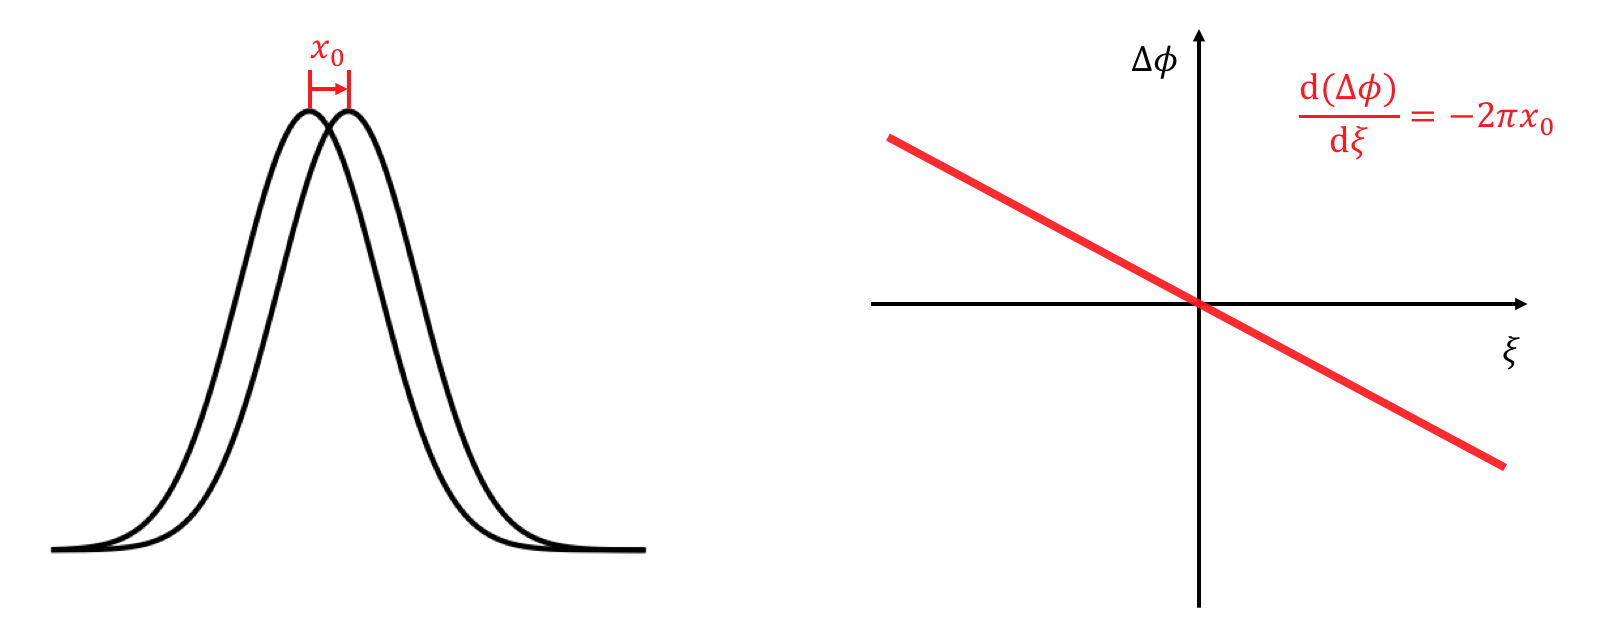
\includegraphics[width = 0.99 \linewidth]
{./Figures/Methods/FT.png}
\caption[Translation property of Fourier transform]
{The left panel shows a signal (or a spectral line profile in the following context) shifted by an amount $x_0$. 
The right panel is the differential phase spectral density diagram (i.e. differential phase spectrum). 
The model shows a perfectly linear correlation 
between $\Delta \phi(\xi)$ and $\xi$ with the constant slope $-2 \pi x_0$.}
\label{fig:FT}
\end{figure} 
%-------------

Let us consider a function $h(x)$ be a signal $f(x)$ delayed (or shifted) by an amount $x_0$:
\begin{equation}
	h(x) = f(x-x_0).
\label{eq:FT1}
\end{equation}
In the frequency domain, we will then have 
\begin{equation}
	\hat{h}(\xi) = e^{-2 \pi ix_0 \xi} \hat{f}(\xi),
\label{eq:FT2}
\end{equation}
where the circumflex denotes the Fourier transform of a function. $\hat{h}(\xi)$ and $\hat{f}(\xi)$ 
will therefore differ by a frequency dependent phase angle: 
\begin{equation}
	\Delta \phi(\xi) = -2 \pi x_0 \xi,
\label{eq:PhaseShift}
\end{equation}
while the power spectral density will remain unchanged (as $\mid e^{-2 \pi ix_0 \xi}\mid ^2 = 1$).



\subsection{Intuitive explanation}

The translation property of the Fourier transform follows mathematically from the nature of the transform. 
A (perhaps) more intuitive way to see this is that since the Fourier transform is defined 
\begin{equation}
	\hat{f}(\xi) = \int_{-\infty}^{\infty} f(x) e^{-2 \pi ix \xi} dx, 
\label{eq:FT3}
\end{equation}
it decomposes the function $f(x)$ into a frequency representation $\hat{f}(\xi)$, such that the function $f(x)$ is expressed  
as the sum of \textit{all} the orthogonal basis $e^{2 \pi ix \xi}$ times a set of their components $\hat{f}(\xi)$ (i.e.
by the inverse Fourier transform):
\begin{equation}
	f(x) = \int_{-\infty}^{\infty} \hat{f}(\xi) e^{2 \pi ix \xi} d\xi. 
\end{equation}

This means that shifting $f(x)$ by $x_0$ is equivalent to shifting \textit{all} the orthogonal basis functions by $x_0$, which becomes $e^{2 \pi i(x-x_0) \xi} = e^{2 \pi i x \xi} \cdot e^{-2 \pi ix_0 \xi}$. This is how the $e^{-2 \pi ix_0 \xi}$ term in Eq.~\ref{eq:FT2} arises -- it quantifies this phase difference. 
\footnote{For a simplified vision bridging a shift of the signal in the time domain and a phase difference in the frequency domain, imagine any real continuous function is a sum of sines and cosines. Changing the phase angle in the sines and cosines results in shifts in the function.}

The fact that the power spectrum density remains the same can also intuitively seen, because shifting the signal as a whole 
doesn't add or remove any frequency information. 


\subsection{Practical Use}

From Eq.~\ref{eq:PhaseShift}, we see that the phase shift $\Delta \phi(\xi)$ is proportional to the frequency $\xi$
with a constant gradient or slope 
\footnote{We use $\Delta$ to refer to the phase difference between a shifted line profile and a unshifted~/~referenced line profile, while the derivative to refer to the response of $\Delta \phi)$ to $\xi$.}
\begin{equation}
	\dv{(\Delta \phi)}{\xi} = -2 \pi x_0
\label{eq:gradient}
\end{equation}
Obtaining this (in principle) is straightforward via a simple linear regression model fit to a plot of $\Delta \phi(\xi)$ versus $\xi$ 
 (see e.g. Fig.~\ref{fig:FT}), so that
\begin{equation}
	x_0 = -\frac{1}{2 \pi}\dv{(\Delta \phi)}{\xi}
\label{eq:line_shift}
\end{equation}

By analogy with the definition of power spectral density, we describe $\phi(\xi)$ the ``phase spectral density'' and hence $\Delta \phi(\xi)$ the ``differential phase spectral density''. 

\paragraph{Concluding remarks}
In principle then, an  analysis of the phase shift in the frequency domain of the Fourier components of
a line profile will provide a means of measuring a bulk line shift in real space. 
% More importantly,
% it may provide a means of separating  an apparent radial velocity shift into the components due to bulk line shift, 
% and line profile shape change.


%----------------------------------------------------------------------------------------	

\subsection{Initial tests}

We performed an initial test to determine whether we can correctly recover known shifts of a line profile  
from an analysis of the phase shift in the frequency domain of the Fourier transform of shifted line profiles.

We generated a spectral line profile based on the cross-correlation function of observed HARPS spectra
with the software SOAP 2.0 {\em CGT: Referece}. This was replicated 100 times, with a very small amount of 
noise (equivalent to a S/N = 10,000 in the line profiles) injected. These profiles were then
subjected to radial velocity shifts evenly spaced between 0 and 10\,m/s (Fig.~\ref{fig:line_profiles12}). 

%-------------
\begin{figure}[tbp]
    \begin{subfigure}[b]{0.49\textwidth}
        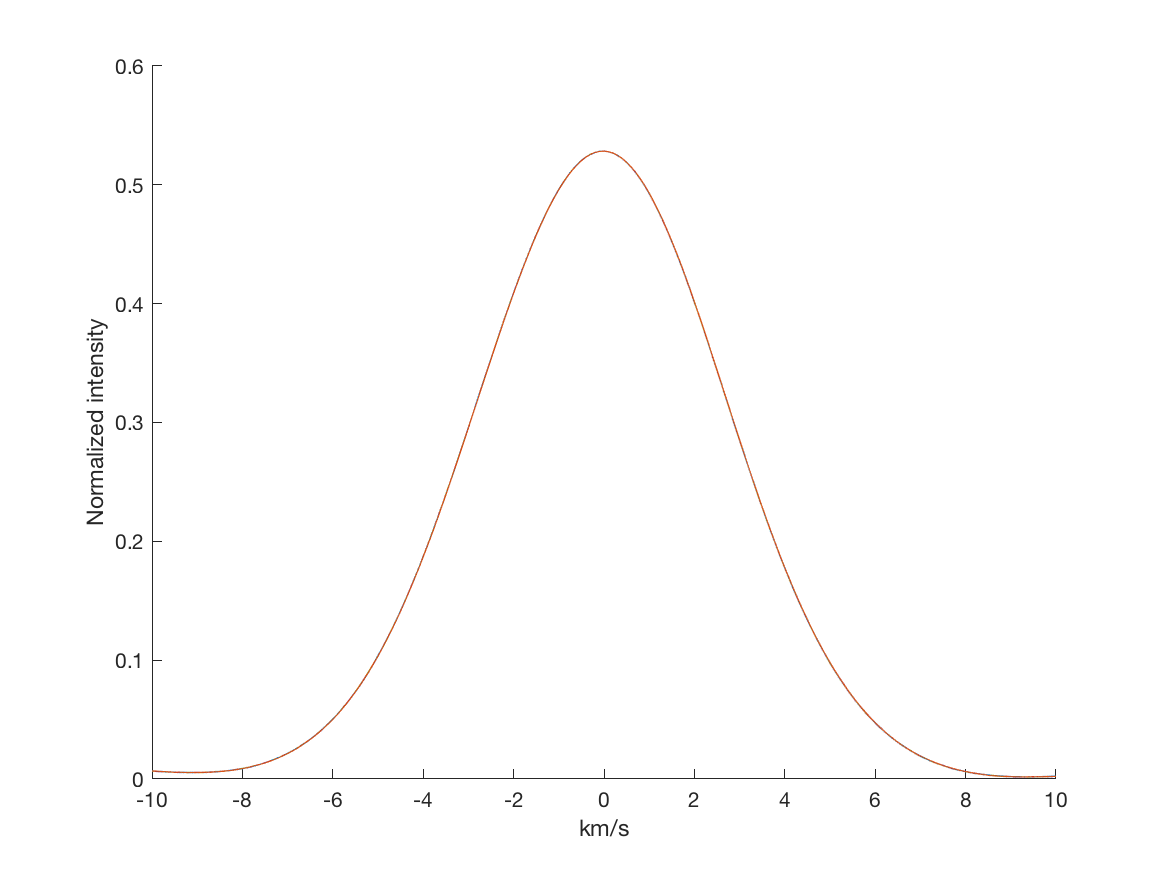
\includegraphics[width=\textwidth]{./Figures/Methods/1-Line_Profile.png}
        \caption{Line profile (stacked)}
        \label{fig:line_profiles}
    \end{subfigure}
	~
    \begin{subfigure}[b]{0.49\textwidth}
        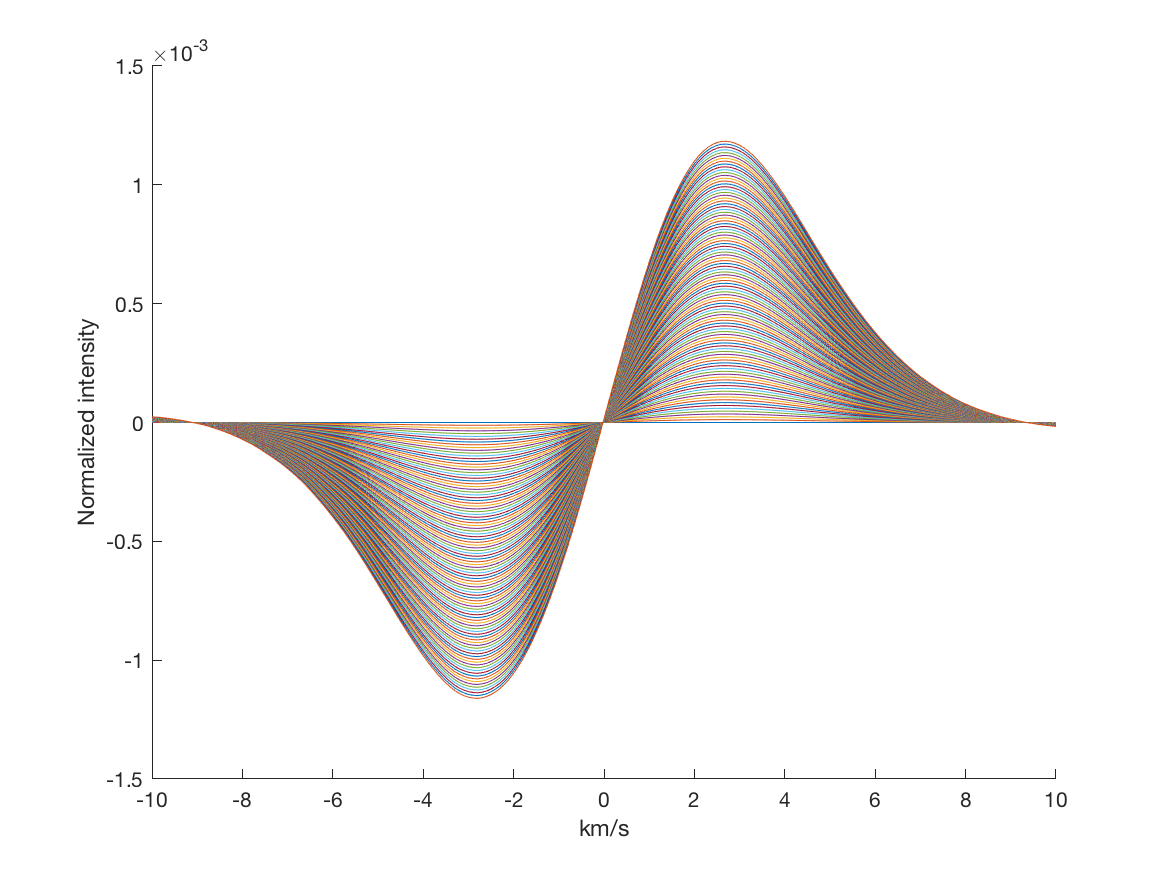
\includegraphics[width=\textwidth]{./Figures/Methods/1-Differential_line_Profile.png}
        \caption{Differential line profile}
        \label{fig:differential_line_profiles}
    \end{subfigure}	
    
    \caption[100 shifted HARPS-like line profiles]{(a) the shifted line profiles plotted on top of each other, showing that 		the $\pm$0-10\,m/s shifts are very small compared to the line profile width. (b) the shifted line profiles with the 			unshifted line profile subtracted from each. Note that for demonstration clarity, noise is not included in this 				differential line profile plot and only 10 out of 100 profiles are presented.}
\label{fig:line_profiles12}
\end{figure}	
%-------------

The Fourier transform of these 100 spectral line profiles divides the information into two parts: 
(1) the power spectra (Fig.~\ref{fig:power_spectrum}) and (2) the phase spectra (shown in Fig.~\ref{fig:dps}
as the differential phase spectra relative to the phase spectrum for the unshifted line profile). 

%-------------
\begin{figure}[tbp]	
    \begin{subfigure}[b]{0.49\textwidth}
        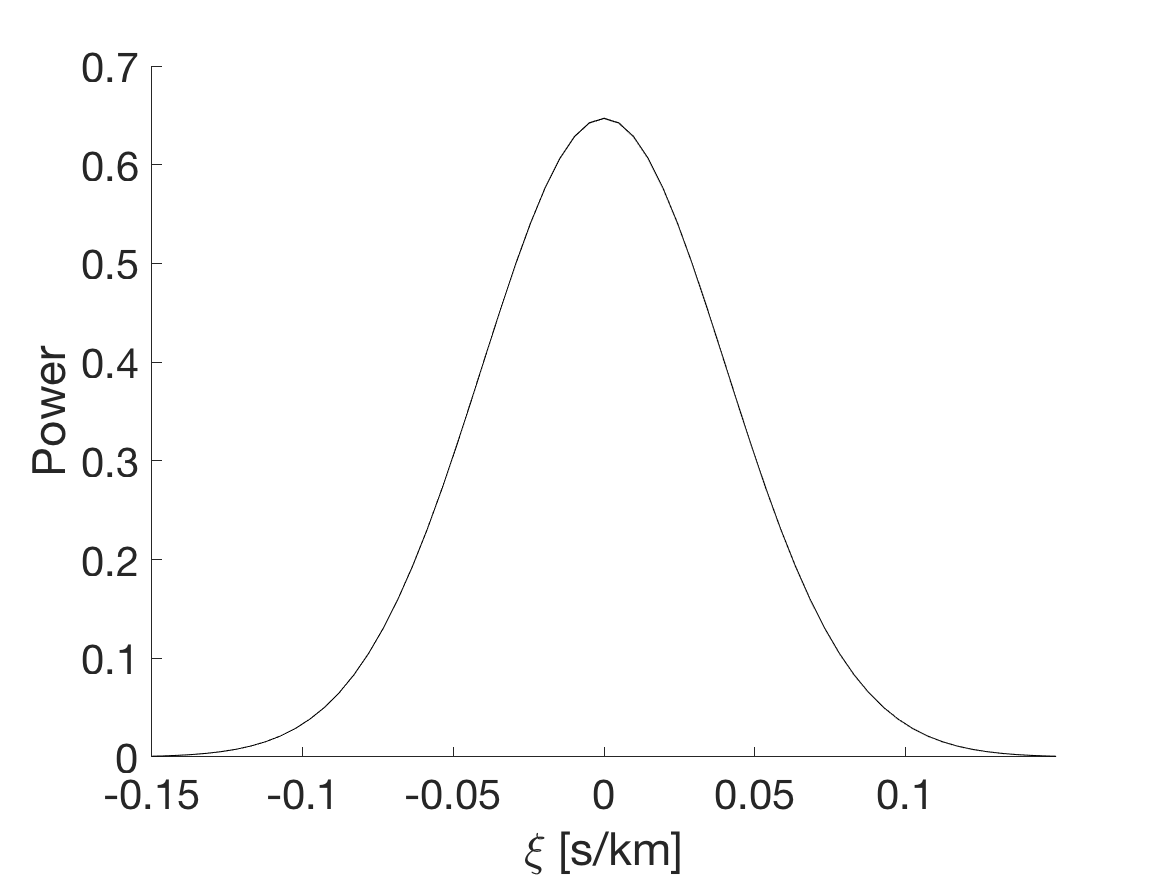
\includegraphics[width=\textwidth]{./Figures/Methods/2-FT_power.png}
        \caption{Power spectrum (stacked)}
        \label{fig:power_spectrum}
    \end{subfigure}
	~
    \begin{subfigure}[b]{0.49\textwidth}
        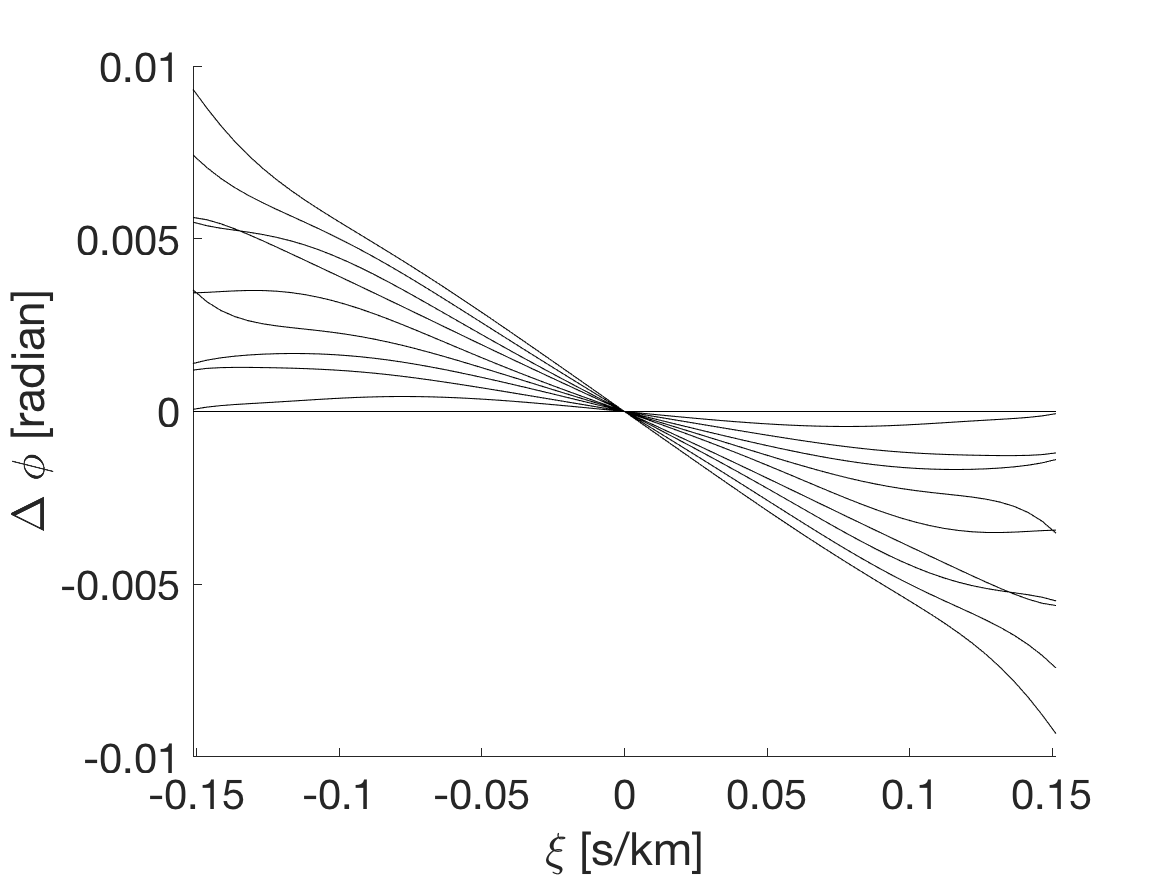
\includegraphics[width=\textwidth]{./Figures/Methods/4-Relative_phase_angle.png}
        \caption{Differential phase spectrum}
        \label{fig:dps}
    \end{subfigure}	
    
    \caption[Fourier transform of 100 shifted line profiles]{The Fourier transform of these shifted line 				profile divides the information in each into (a) their power spectra and (b) their phase spectra (here	 			plotted differential compared to that 	of the unshifted profile). A line shift in the time domain 				produces an unchanged power spectrum in the frequency domain. It does, however, produce phase shift which 			we see as linear trends in the differential phase spectra as a function of frequency. Note that for 				demonstration clarity, only 10 out of 100 differential phase spectra are presented.}
\label{fig:FT_process}
\end{figure}    
%-------------

{\em CGT: whereas the frequency ranges plotted in 2,.2a and 2.2b are the same [are they really? are you sure the axis on 2.2b should not be in m/s instead of km/s?]
, the ranges plotted in 2.3a and 2.3b are different. You don't really say why. Until later when you make comments about "noise".
I suggest you should make both the plots over the same range, and then *point out* the impact of noise,
and why you have chosen to limit your fits to a smaller frequency range (and justify that choice),}

We see that most Fourier transform information is concentrated in the lower frequency range in the power spectrum.
The differential phase spectra are expected linear (as Fig.~\ref{fig:FT} demonstrated). Its deviation from linearity 
comes from the noise that we injected, which will be discussed later. 

The slope of each differential phase spectrum indicates the shift of each line profile relative to 
the unshifted line profile. It should be weighted by the amplitude of the power, meaning the lower frequencies 
are higher weighted. We therefore calculate the radial velocity shift for each shifted line profile
using two methods: 
\begin{enumerate}
	\item the $RV_\text{FT}$ using Eq.~\ref{eq:line_shift}, weighted by the power spectrum
	\item the $RV_\text{Gaussian}$ as traditionally measured from the line centroid by fitting a Gaussian to each line profile.
\end{enumerate}
We can then compare the results with the (known) input line shift where we see the expected strong 1:1 correlation (Fig.~\ref{fig:rv_recovery}). The root-mean-square (rms) of the residuals are both $rms_\text{FT} = rms_\text{Gaussian} = 0.08$ m/s, identical up to two decimal places, indicating the expected radial velocities are consistently reduced. In addition, the fact that the two methods are so coherently different from the input radial velocity (by a small amount), as shown in the residual of Fig.~\ref{fig:rv_recovery}, means that such deviation comes from the photon noise intrinsic to the line profile rather than the methods themselves. 

{\em CGT: How do these comare which what you'd expect from the S/N and the intrinsic line width (should say at some int what the intrinsic line width is}.

%-------------
\begin{figure}[tbp]
\centering
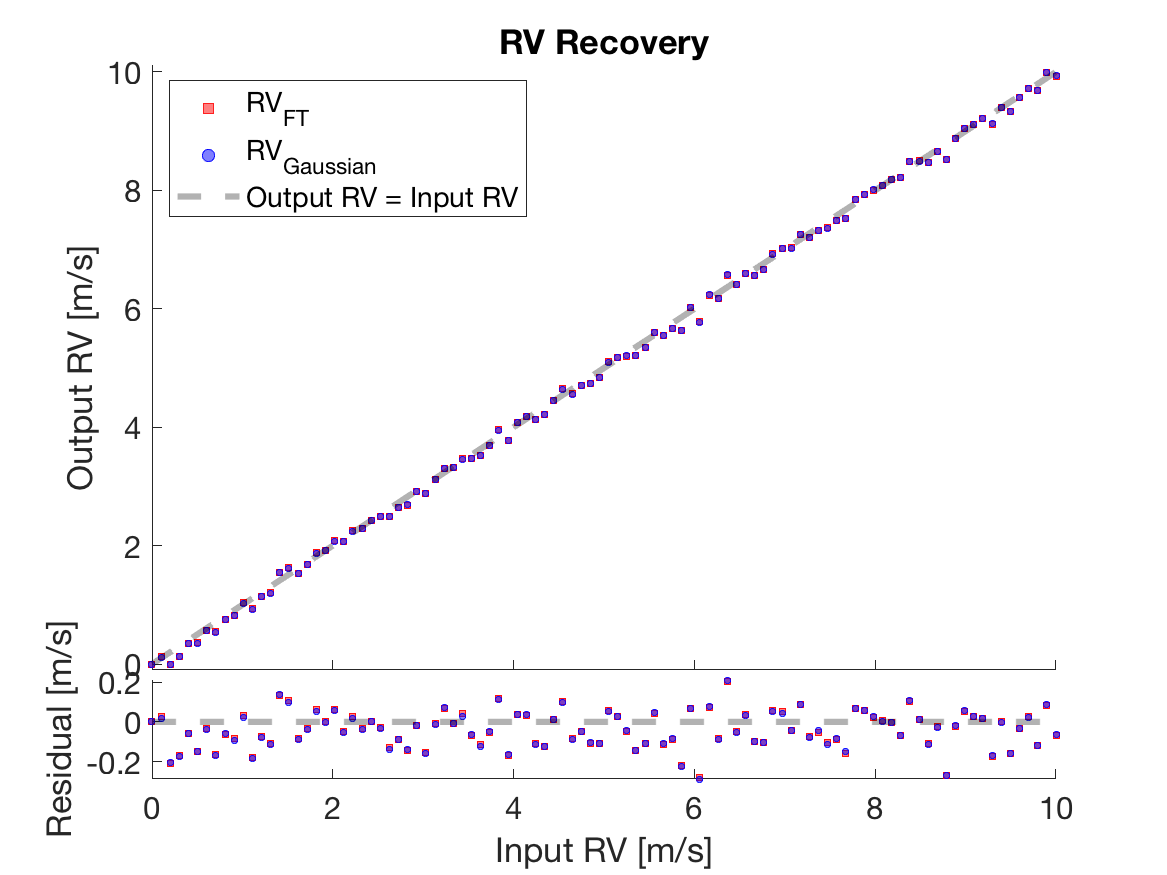
\includegraphics[width = 0.7 \linewidth]
{./Figures/Methods/5-LINE_SHIFT_ONLY.png}
\caption[Radial velocity recovery]
{Radial velocity recovery of line shifts with both methods: Fourier transform and Gaussian fit. Both results are highly consistent with each other.}
\label{fig:rv_recovery}
\end{figure} 
%-------------

\paragraph{Impact of noise}
We briefly mentioned above that the deviation from linearity in the differential phase spectrum arises from the photon noise  injected in the simulated line profile. This can be explained with the Fourier transformed line profile $\hat{h}(\xi)$ in a complex plane (also known as the Argand plane; Fig.~\ref{fig:FT_compelx_plane}). What we see is $\hat{h}(\xi)$ literally plotted on the complex plane -- of each complex number $\hat{h}(\xi)$, the argument returns the phase angle and the square of the absolute value returns the power, for that particular frequency $\xi$. For larger powers ($\hat{h}(\xi)$ far from the origin), the presence of noise hardly alters the phase angle; for lower powers ($\hat{h}(\xi)$ distributed in the vicinity of the origin), a slight displacement of $\hat{h}(\xi)$ in the complex plane means a considerable change in the phase angle. It justifies using the Fourier transform spectral power to be the weight of each frequency, and introducing a cut-off frequency when making a linear fit of the differential phase spectrum. 

%-------------
\begin{figure}[tbp]	
    \begin{subfigure}[b]{0.49\textwidth}
        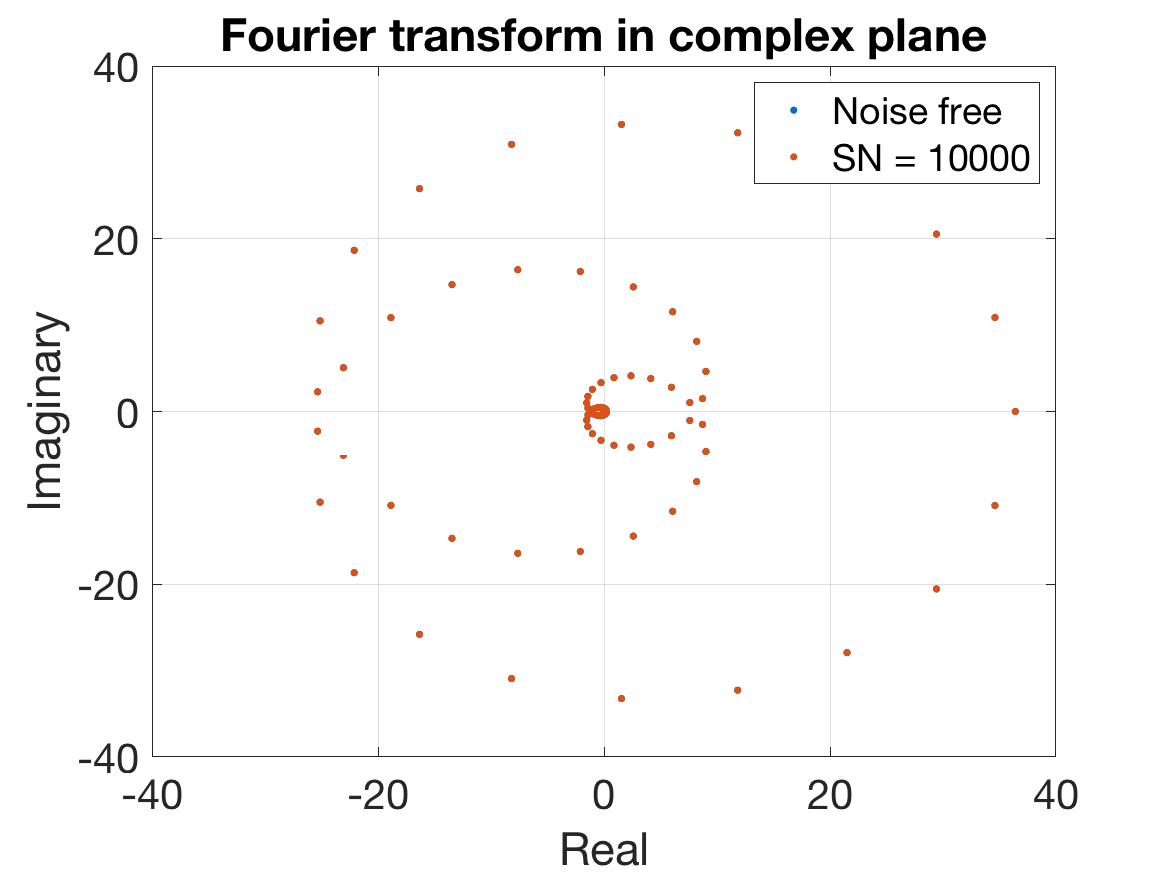
\includegraphics[width=\textwidth]{./Figures/Methods/7-Phase_angle_in_complex_plane_1.png}
%        \caption{Power spectrum (stacked)}
        \label{fig:FT_compelx_plane_1}
    \end{subfigure}
	~
    \begin{subfigure}[b]{0.49\textwidth}
        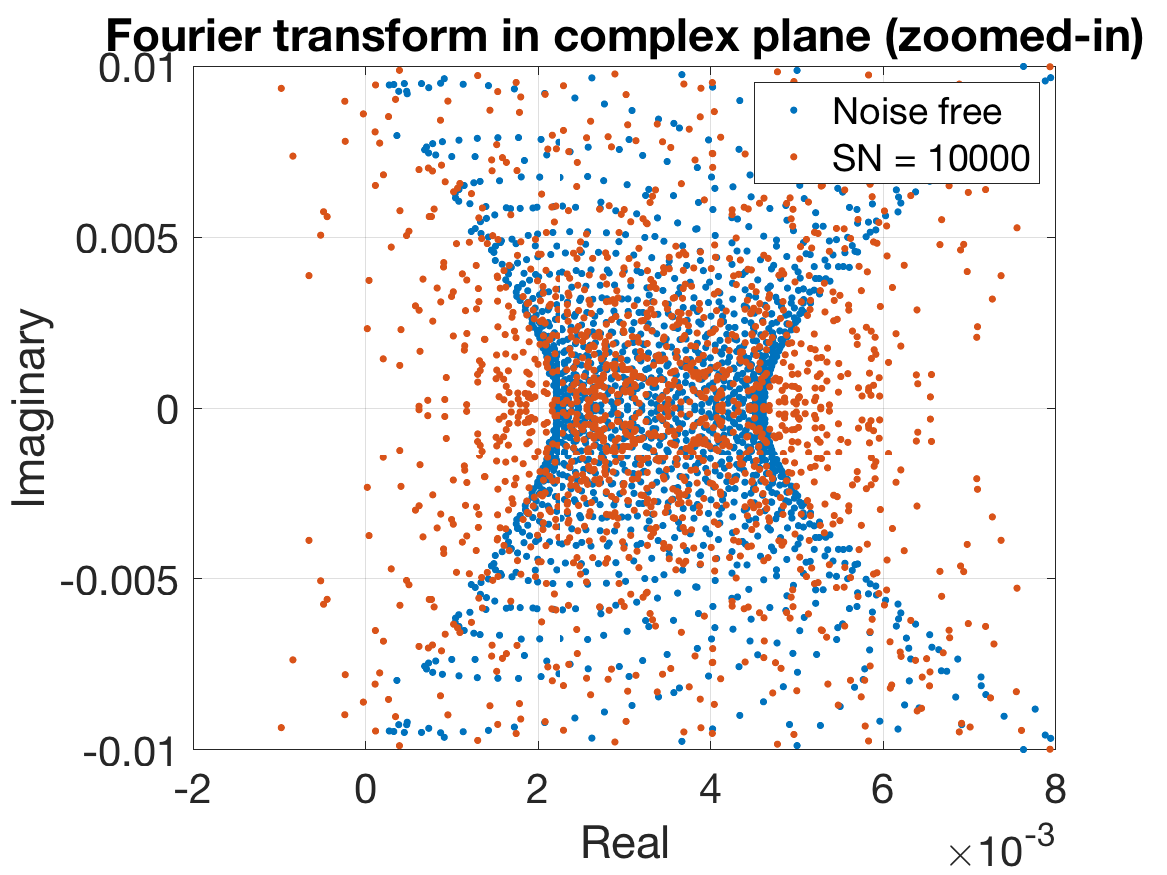
\includegraphics[width=\textwidth]{./Figures/Methods/7-Phase_angle_in_complex_plane_2.png}
%        \caption{Differential phase spectrum}
        \label{fig:FT_compelx_plane_2}
    \end{subfigure}	
    
    \caption[Fourier transform of a line profile in a complex plane]
    {The Fourier transform of a line profile in a complex plane. }
\label{fig:FT_compelx_plane}
\end{figure}    
%-------------

%This is because we only use part of the information from the original line profile -- both because we utilise a limited range of the differential phase spectra, and because we use only the phase spectra to measure this shift (ignoring the power spectra), while the total information in the original shifted line profile is contained in the combination of the power and phase spectra. 
%
%{\em CGT: This needs more work. You need to show the region you are not using to explain why you choose a more linited range, and
%then say why you chose that more limited range and justify it. Don't just say "higher frequency}.
%
%In fact, higher frequency range becomes useless 
%as the interpretation of Fourier transform in high frequencies is dominated by noise and does not represent the 
%intrinsic shift of the line profile any more. As a result, linearity of phase spectrum breaks down in higher frequencies. 
%The range of ``useful" frequencies will depend on the amount of noise (i.e. S/N). 



\paragraph{Concluding remarks}
These initial  tests confirm our expectation --  it is possible to measure a radial velocity from
the Fourier phase spectrum, and this provides an alternative to the traditional 
means of obtaining the radial velocities via centroiding the line profile in real space. 
In a broader context, this method will be applicable to measuring shifts of any pattern, and  
can be extended to higher dimensions. In this thesis, we primarily focus on its use to measure radial velocity shifts in spectral line profiles, and especially whether the Fourier transform phase velocity is more
robust against the influence of changes in line deformation than traditional techniques.

%----------------------------------------------------------------------------------------	

\section{Using the Fourier transform to probe line deformation}
\label{\thesection}
\label{sec:FT_ld}


\subsection{Theory}
\label{sec:LD_Theory}

We wish to test whether this new method for measuring radial velocities is more
robust against spurious apparent radial velocity shifts produced by changes in the
line profile shape in an emitting stars, rather than actual line profile shifts due to a bulk motion
of the emitting star.
In \S~\ref{ch:FT_line_shift}, the same shift $x_0$ applies to \textit{all} the basis functions. 
In the case of line deformation due to stellar variability, $x_0$ becomes frequency dependent 
\footnote{excluding the case where the result of a line deformation is exactly the same as a line shift, as 
this becomes indistinguishable by any means}. That is to say, basis functions at different frequencies would 
shift by different amounts, resulting in shape changes (e.g. skewness) in the line profile. 
Therefore we modify the translation property of Fourier transform
by rewriting $x_0$ as $x_0(\xi)$ in Eq.~\ref{eq:PhaseShift}:
\begin{equation}
	\Delta \phi(\xi) = -2 \pi x_0(\xi) \xi.
\label{eq:PhaseShift2_LPD}
\end{equation}
As a result, the local gradient of the differential phase spectrum becomes 
\begin{equation}
	\dv{(\Delta \phi)}{\xi} = -2 \pi (x_0 + \dv{x_0}{\xi}),
\label{eq:PhaseShift3_LPD}
\end{equation}
which reduces to Eq.~\ref{eq:gradient} when $x_0$ is a constant as in the case of a bulk line shift.
Note that the dependency of $\xi$ has been taken out of $\Delta \phi(\xi)$ and 
$x_0(\xi)$ in writing the differential equation above. 

In principle, we could numerically solve this differential equation based on the measured local gradient d$(\Delta \phi)$/d$\xi$
to obtain $x_0(\xi)$. As a simplistic approach, if $x_0(\xi)$ changes with $\xi$ slowly within a certain frequency range,
we can make the approximations that $x_0\sim$~const and d$x_0$/d$\xi\sim0$. With this, Eq.~\ref{eq:PhaseShift3_LPD} 
converges back to Eq.~\ref{eq:gradient}.

\subsection{SOAP Simulations}
\label{sec:Simulations}


With SOAP~2.0, we injected three spots with different longitudes, latitudes and sizes (Table~\ref{table:spot_configurations}) to model an emitting star, and generate 100 cross-correlation functions for the resulting  deformed line profiles evenly sampled throughout the rotation period of the star (Fig.~\ref{fig:line_profiles_deformation}). A very small amount of noise (equivalent to a S/N = 10,000) was also added into the line profiles. We then take the same approach as in  \S~\ref{ch:FT_line_shift} to obtain the power spectrum and (differential) phase spectrum (Fig.~\ref{fig:FT_process_LPD}) to recover the radial velocities $RV_\text{FT}$. It notes, line deformation contributes to a skewed differential phase spectrum, as predicted in \S\ref{sec:LD_Theory}. 

%-------------
\begin{table}[htbp]
\centering
\begin{tabular}{|c|c|c|c|}
\hline 
 & Longitude & Latitude & Size in disk area percentage\\ 
\hline 
Spot 1 & $174^\circ$ & -$14^\circ$ & 0.18\% \\ 
\hline 
Spot 2 & $288^\circ$ & $74^\circ$  & 0.40\% \\ 
\hline 
Spot 3 & $51^\circ$  & $52^\circ$  & 0.50\% \\ 
\hline 
\end{tabular} 
\caption{Spot configurations}
\label{table:spot_configurations}
\end{table}
%-------------

%-------------
\begin{figure}[tbp]
    \begin{subfigure}[b]{0.49\textwidth}
        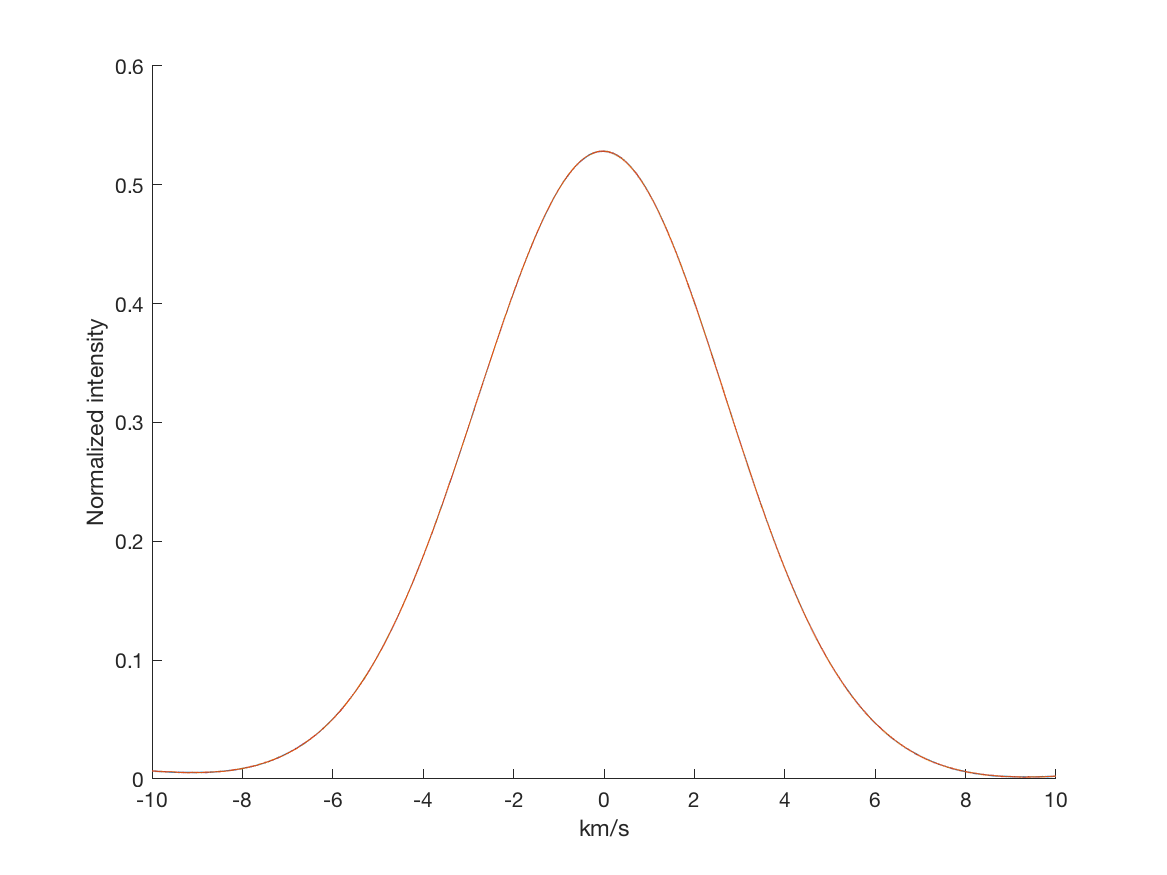
\includegraphics[width=\textwidth]{./Figures/Methods/LPD1-Line_Profile.png}
        \caption{Line profile (stacked)}
    \end{subfigure}
	~
    \begin{subfigure}[b]{0.49\textwidth}
        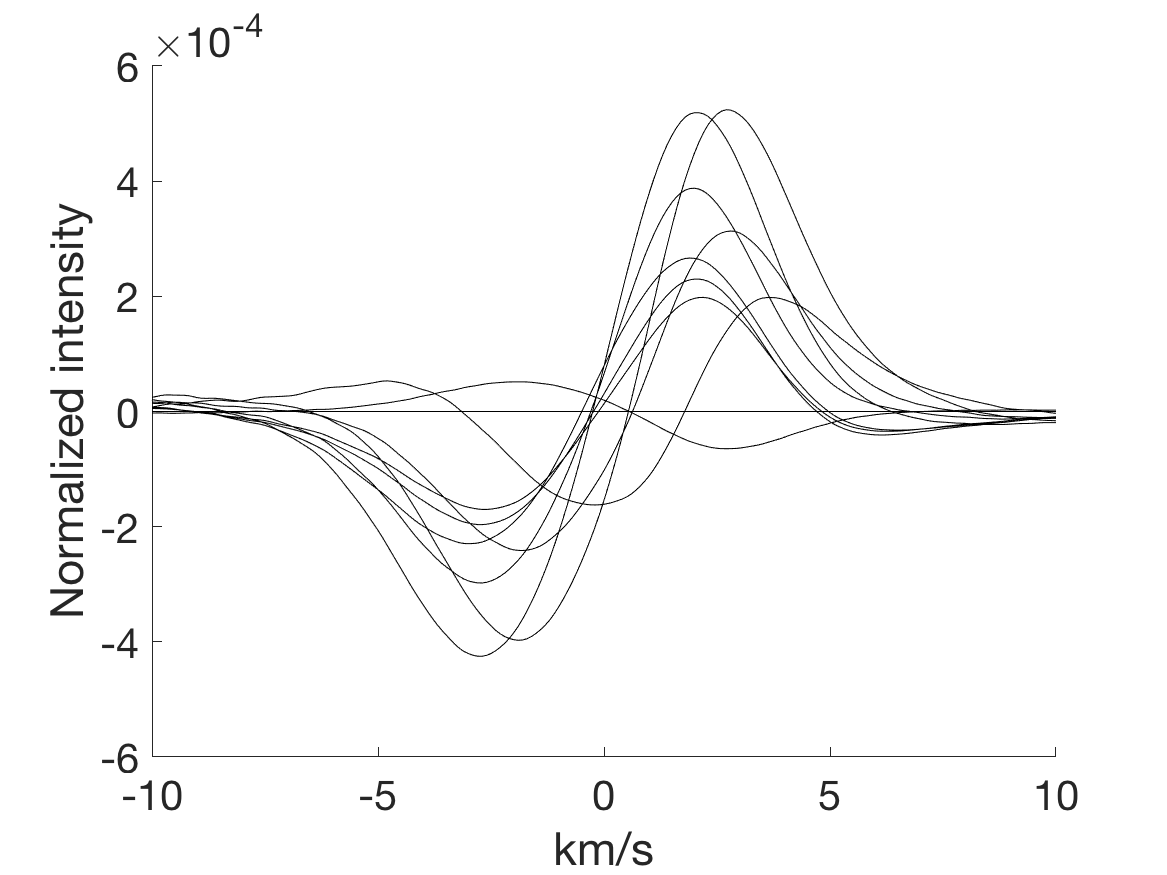
\includegraphics[width=\textwidth]{./Figures/Methods/LPD1-Differential_line_Profile.png}
        \caption{Differential line profile}
        \label{fig:ld_dlp}
    \end{subfigure}	
    
    \caption[Deformed line profile]{Deformed line profile. For the sake of clarity, noise is not included in  
    the differential line profile plot and only 10 out of 100 profiles are presented.}
\label{fig:line_profiles_deformation}
\end{figure}	
%-------------

%-------------
\begin{figure}[tbp]	
    \begin{subfigure}[b]{0.49\textwidth}
        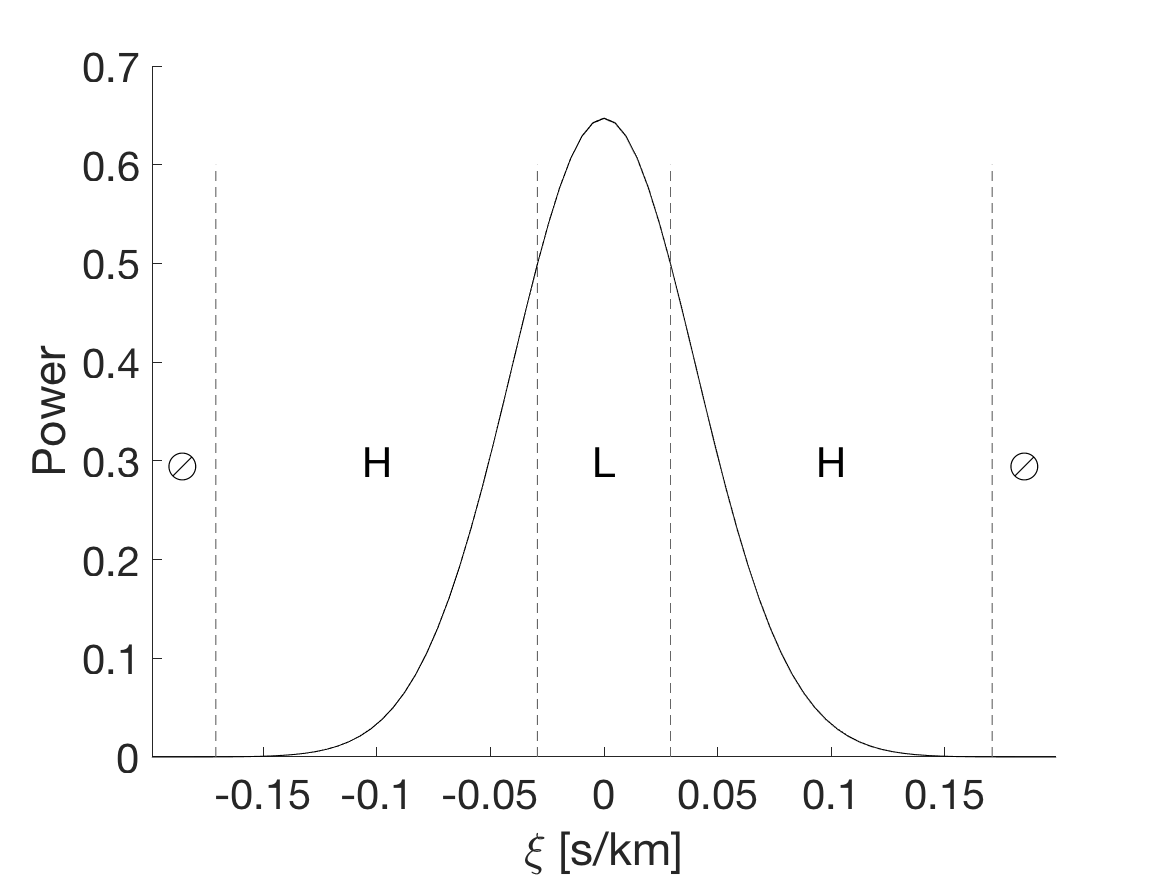
\includegraphics[width=\textwidth]{./Figures/Methods/LPD2-FT_power.png}
        \caption{Power spectrum (stacked)}
    \end{subfigure}
	~
    \begin{subfigure}[b]{0.49\textwidth}
        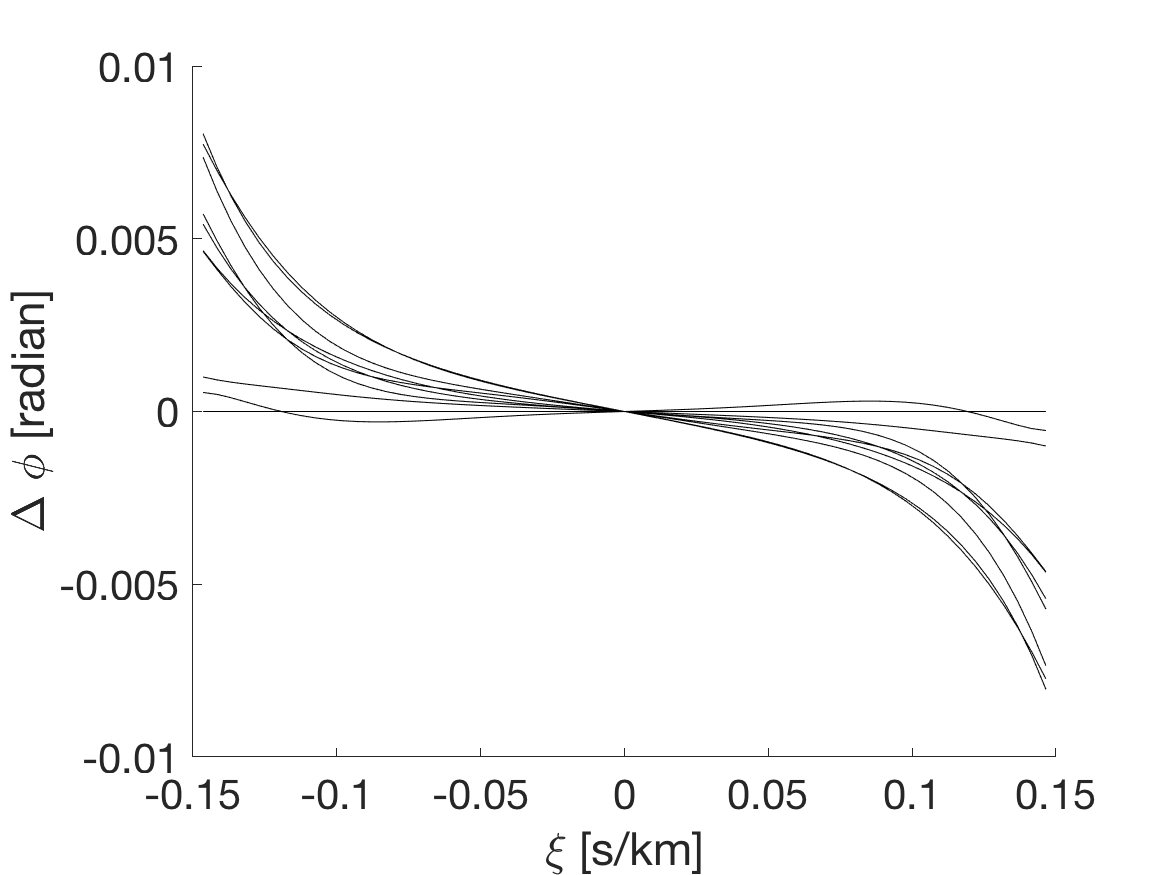
\includegraphics[width=\textwidth]{./Figures/Methods/LPD4-Relative_phase_angle.png}
        \caption{Differential phase spectrum}
        \label{fig:dps_LPD}
    \end{subfigure}	
    
    \caption[Fourier transform of deformed line profile]
    {Fourier transform of deformed line profile. Only 10 out of 100 differential phase spectra are presented.}
\label{fig:FT_process_LPD}
\end{figure}    
%-------------

In this case, the input radial velocities would be the apparent radial velocities of deformed line profiles (also known as jitter). Both velocities $RV_\text{FT}$ and $RV_\text{Gaussian}$ are plotted against rotation phase (Fig.~\ref{fig:rv_recovery_deformed}). If we take the root-mean-squares of both $RV_\text{FT}$ and $RV_\text{Gaussian}$ to be the intrinsic noise level ($rms_\text{FT} = rms_\text{Gaussian} = 0.08$ m/s) corresponding S/N = 10,000, the uncertainty of $RV_\text{FT} - RV_\text{Gaussian}$ as residual would have an uncertainty of $\sqrt{rms_\text{FT}^2+rms_\text{Gaussian}^2}\approx0.11$ m/s, meaning that the residuals are 0 within uncertainty and showing that $RV_\text{FT}$ and $RV_\text{Gaussian}$ are indistinguishably consistent. 

%-------------
\begin{figure}[tbp]
\centering
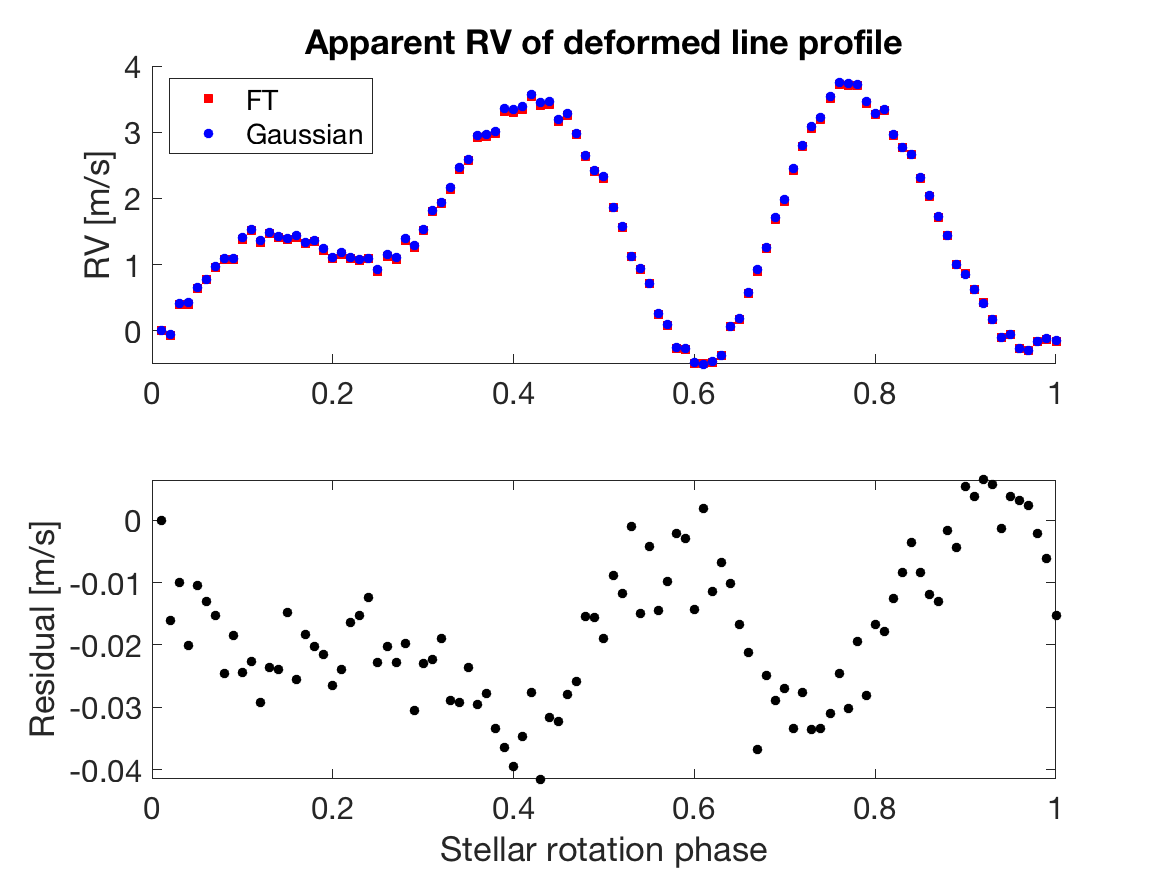
\includegraphics[width = 0.7 \linewidth]
{./Figures/Methods/5-JITTER_ONLY_3.png}
\caption[Apparent RV of deformed line profile]
{Apparent RV of deformed line profile calculated with Fourier transform and Gaussian fit. Both results are also highly consistent with each other.}
\label{fig:rv_recovery_deformed}
\end{figure} 
%-------------

\paragraph{Remark} Using (almost) all the information in the power spectrum and the phase spectrum will end up with the same radial velocity as acquiring the line centroid fitted by a Gaussian line profile. 

Although the intrinsic line deformation (in the absence of any velocity shift in the host star) does mimic the radial velocity shift, we note the shape and scale differences in the differential phase spectrum between an actual line shift (Fig.~\ref{fig:FT_process}) and a line deformation (Fig.~\ref{fig:FT_process_LPD}) -- the latte becomes highly skewed as $\mid\Delta \phi\mid$ increases dramatically towards higher frequencies. Such differences provide key messages to differentiate the two circumstances. 

For example, as Fig.~\ref{fig:low-high-pass} presents, if we divide (arbitrarily) the frequencies into low frequency range ($\mid\xi\mid<0.06$ s/km; i.e. apply a low-pass filter) and high frequency range ($\mid\xi\mid>0.06$ s/km; i.e. apply a high-pass filter)\footnote{In this example, we limit the higher frequency range effective in 0.06 s/km $<\mid\xi\mid<0.15$ s/km, because frequencies higher than 0.15 s/km hardly contributes to the shape of the line profile (the power $\sim$ 0), and they are also heavily impacted by noise.}, and compute the equivalent Fourier transformed radial velocity $RV_\text{FT}$ for each, we would obtain two sets of radial velocities, one represents the radial velocity shifts (denoted as $RV_\text{FT,L}$) of the lower frequency components and the other (denoted as $RV_\text{FT,H}$) represents the higher. 

%-------------
\begin{figure}[tbp]	
    \begin{subfigure}[b]{0.49\textwidth}
        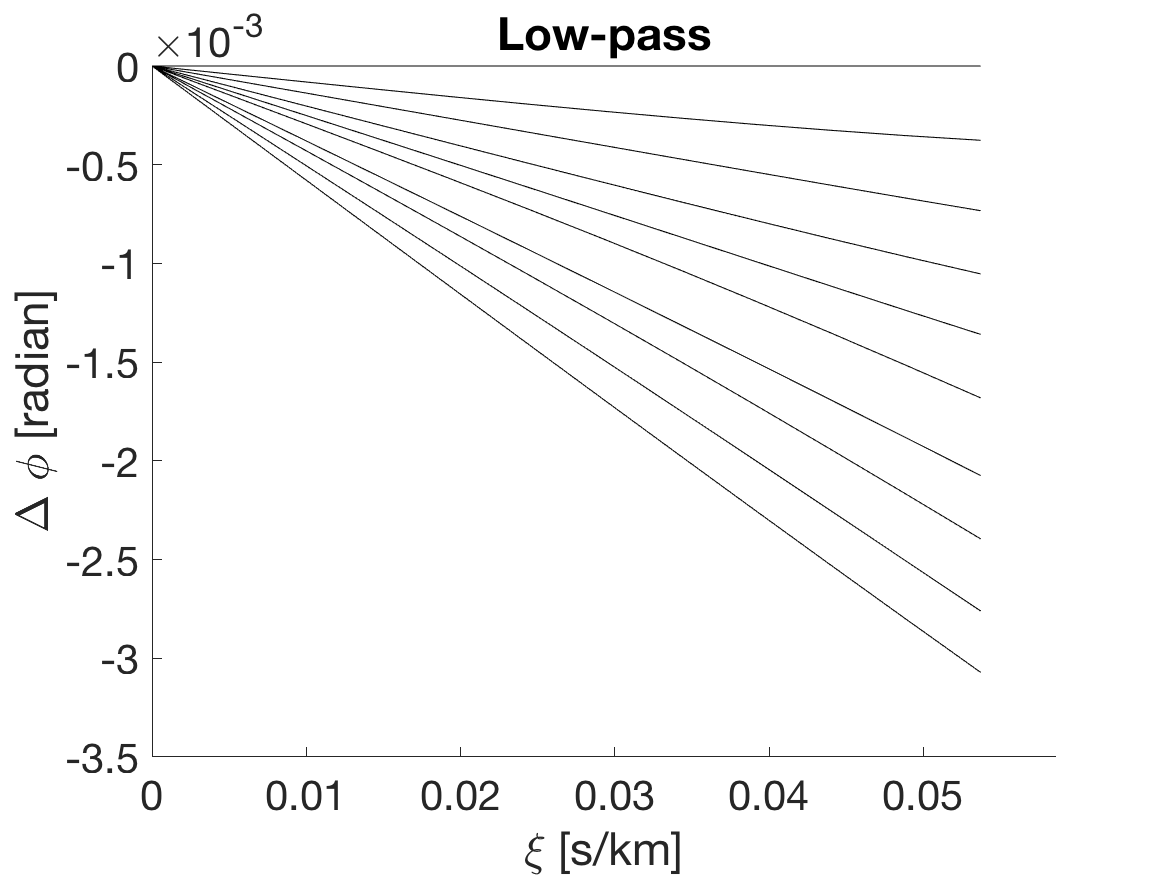
\includegraphics[width=\textwidth]{./Figures/Methods/4-Relative_phase_angle_L.png}
%        \caption{Power spectrum (stacked)}
    \end{subfigure}
	~
    \begin{subfigure}[b]{0.49\textwidth}
        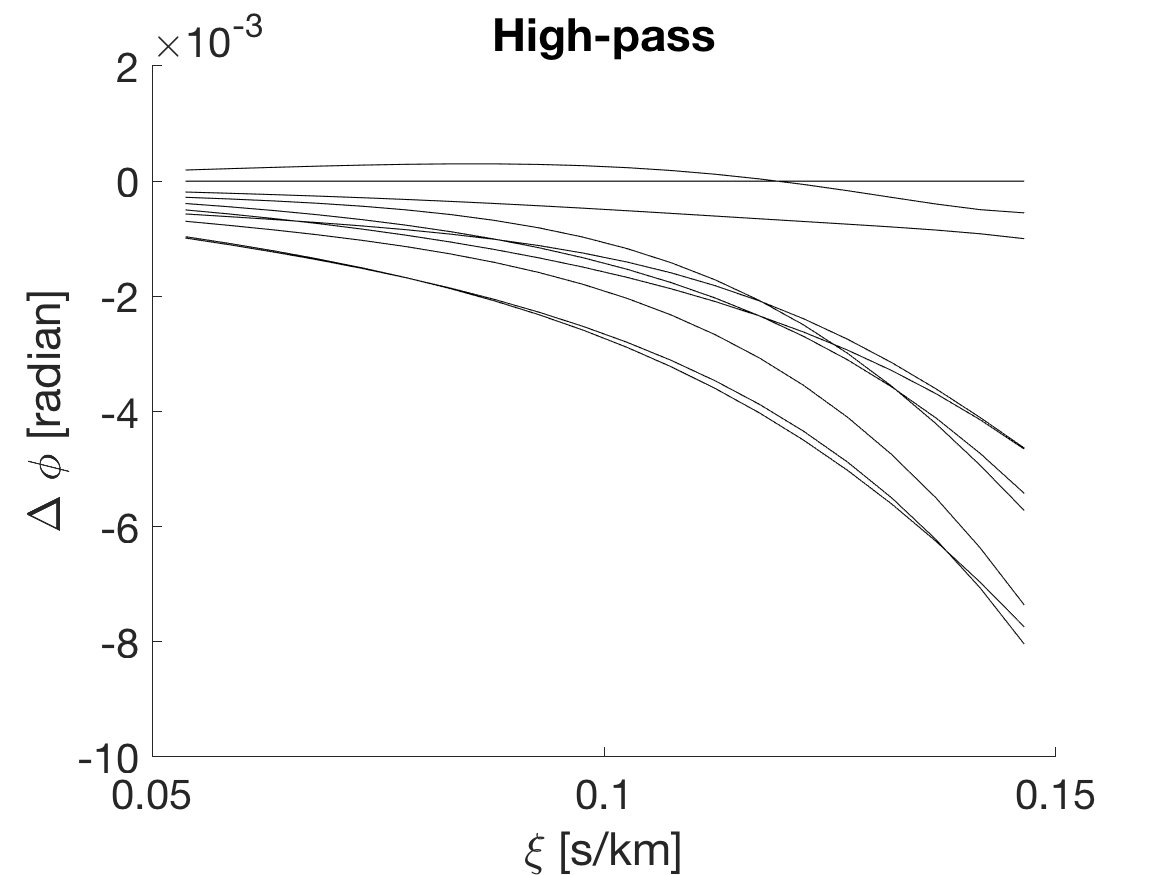
\includegraphics[width=\textwidth]{./Figures/Methods/4-Relative_phase_angle_H.png}
%        \caption{Differential phase spectrum}
    \end{subfigure}	
    
    \caption[Low-pass and high-pass filters]
    {Differential phase spectrum as shown in Fig.~\ref{fig:dps_LPD} sub-divided into lower frequency range and higher frequency range. Only the non-negative ranges are plotted.}
\label{fig:low-high-pass}
\end{figure}    
%-------------

We find, to our surprise, that both $RV_\text{FT,L}$ and $RV_\text{FT,H}$ are linearly correlated with the jitter (equivalent to $RV_\text{Gaussian}$ in this case as no planets are present; Fig.~\ref{fig:FT_vs_Gaussian}), yet neither has a 1:1 correlation -- $RV_\text{FT,H}$ demonstrates a higher response to jitter, with a slope $k_\text{H} = 1.8599$ in the linear fit, meaning the radial velocity shift of 1 m/s due to line deformation is detected as 1.8599 m/s shift on average using \textit{this} high-pass filter; whereas $k_\text{L} = 0.8245$ for $RV_\text{FT,L}$, meaning such a 1 m/s deformation is detected as 0.8245 m/s shift on average using \textit{this} low-pass filter. When we combine both filters, we would have obtained the 1:1 correlation as discussed above (Fig.~\ref{fig:rv_recovery_deformed}).

%-------------
\begin{figure}[tbp]
\centering
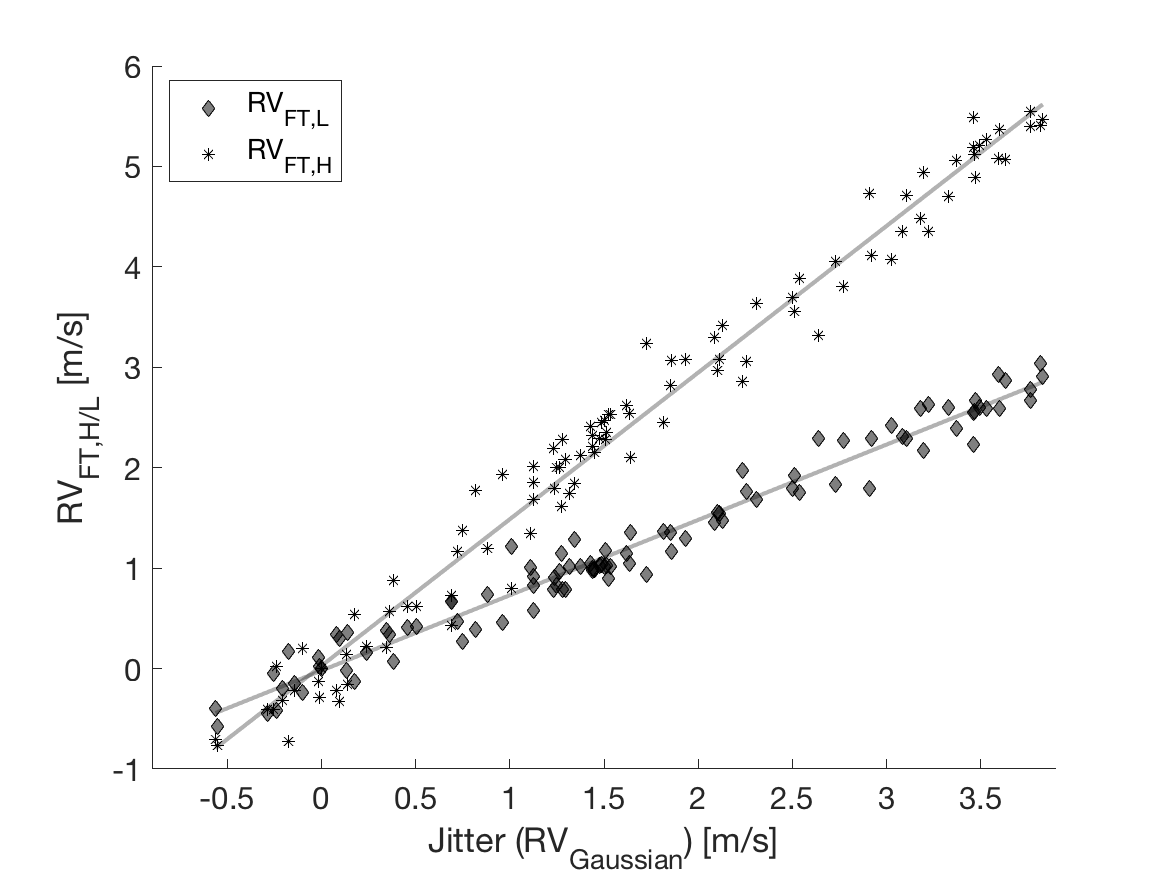
\includegraphics[width = 0.7 \linewidth]
{./Figures/Methods/5-JITTER_ONLY_1.png}
\caption[Fourier transform in response to line deformation]
{Applying the low-pass and high-pass filters, the Fourier transform $RV_\text{FT,L}$ and $RV_\text{FT,H}$ are linearly correlated with the jitter ($RV_\text{Gaussian}$).}
\label{fig:FT_vs_Gaussian}
\end{figure} 
%-------------

We could further investigate how well this linearity behaves for each filter by scaling the measured $RV_\text{FT,L}$ and $RV_\text{FT,H}$ by their corresponding factors $1/k_\text{L}$ and $1/k_\text{H}$ respectively, and compare them with the jitter ($RV_\text{Gaussian}$), as presented in Fig.~\ref{fig:scaling_RV_FT}. The root-mean-squares of the residuals ($RV_\text{FT,L/H} - RV_\text{Gaussian}$) are $rms_\text{FT,L} \approx 0.15$ m/s and $rms_\text{FT,H} \approx 0.32$ m/s respectively. Not surprisingly, $rms_\text{FT,H} > rms_\text{FT,L}$, because in \textit{this} case more information is concentrated in the low-pass filter (i.e. $\int_{0}^{0.05} \mid P \mid d\xi > \int_{0.05}^{0.15} \mid P \mid d\xi$ where $P$ is the amplitude of the power spectrum). For this reason, $rms_\text{FT,L}-RV_\text{Gaussian}$ would be more stable and less scattered. If the bound between the low- and high-pass filer $\xi_0$ is chosen such that $\int_{0}^{\xi_0} \mid P \mid d\xi = \int_{\xi_0}^{0.15} \mid P \mid d\xi$, we would expect $rms_\text{FT,H} = rms_\text{FT,L}$. 

%-------------
\begin{figure}[tbp]
\centering
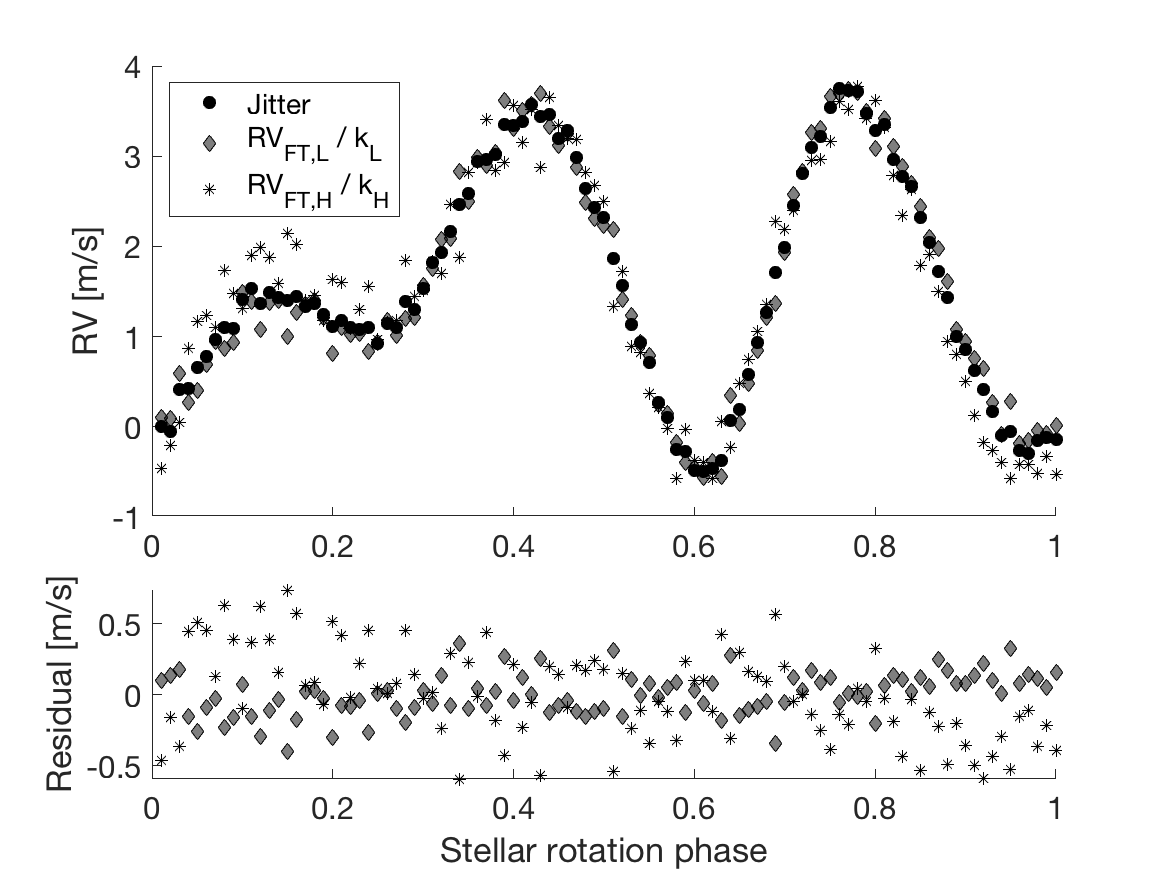
\includegraphics[width = 0.7 \linewidth]
{./Figures/Methods/5-JITTER_ONLY_4.png}
\caption[Scaling the low-pass and high-pass Fourier transformed radial velocities]
{Scaling the low-pass and high-pass Fourier transformed radial velocities to match the input jitter.}
\label{fig:scaling_RV_FT}
\end{figure} 
%-------------

\paragraph{Remark} The apparent radial velocity shift due to spectral line deformation (i.e. jitter) can be seen as a mingle of one radial velocity shift in higher frequency components and one in lower frequency components. They are both, in the SOAP simulations, scaled with the jitter. 

%An intuitive way to understand why 
%
%If we compare the differential phase spectra in Fig.~\ref{fig:FT_process} and Fig.~\ref{fig:FT_process_LPD},
%it is quite obvious that the differential phase spectrum of a deformed line profile is no longer linear 
%due to the $x_0$ dependency on $\xi$, as we discussed in \S~\ref{sec:LD_Theory}. Nevertheless, applying the 
%local linear approximation can provide a radial velocity shift for that frequency range. We will primarily 
%use the lower frequency range (from -0.06 to 0.06~(km/s)$^{-1}$ in this case) for the reasons that 
%it is where information is mostly concentrated and that it is less noise-sensitive. {\em CGT: Sorry, 
%but you still haven't demonstrated this sufficiently}
%
%However, the differential phase shift at lower frequency is {\em less} sensitive to the
%influence of line profile deformation. 
%If we concentrate on frequencies in the range $\mid\xi\mid < 0.06$ (km/s)$^{-1}$ (sensitive to line profile
%structure at  velocities $> 1/\mid\xi\mid = 16$ km/s) we find that these lower frequency modes are
%less effectively modulated by the higher frequency line deformations, as shown in the 
%differential line profile in Fig.~\ref{fig:ld_dlp}. 
%
%In addition, the slope $k$ will change depending on the 
%frequency range in which the linear regression model is applied. 
%For example, if we select the higher frequency range in the differential phase spectrum, we will 
%expect larger $RV_\text{FT}$ and hence a larger $k$ in general. 
%
%{\em CGT: I tried to rewrite the above, but I'm not convinced either the text or the figures are
%very clear! In partiuclar you need a clear and compelling demosntration why you've chosen the lower
%frequency range you have}



\subsection{Jitter model}

We have found in \S~\ref{ch:FT_line_shift} that $RV_\text{FT}$ and $RV_\text{Gaussian}$ demonstrate basically the same response to line shifts. For its linearity in the differential phase spectrum as a result of a line shift (Fig.\ref{fig:dps}), we can interpolate the conclusion to part of the differential phase spectrum, that is, both $RV_\text{FT,H}$ and $RV_\text{FT,L}$ will also have the same response as $RV_\text{Gaussian}$ to a line shift. 
We have also found earlier in this section (\S~\ref{sec:FT_ld}) that $RV_\text{FT,L}$ 
{\em CGT: What range compared to, say, the line width of the line profile?} 
is less sensitive ($k_\text{L} = 0.8245$) to line deformation than $RV_\text{Gaussian}$, whereas $RV_\text{FT,H}$ is more sensitive ($k_\text{H} = 1.8599$).

We can therefore write the following measurable quantities -- $RV_\text{FT,L/H}$ and $RV_\text{Gaussian}$ --
as the sum of corresponding contributions from a bulk shift in the star (which
we hereafter assume to be due to a planet or planets), and variability in the stellar line
profile (hereafter lumped under the general name ``jitter''):
\begin{equation}
	RV_\text{Gaussian} = RV_\text{planet} + RV_\text{jitter},
\label{eq:RV_Gaussian}
\end{equation}
\begin{equation}
	RV_\text{FT,L} = RV_\text{planet} + k_L \cdot RV_\text{jitter},
\label{eq:RV_FT,L}
\end{equation}
and 
\begin{equation}
	RV_\text{FT,H} = RV_\text{planet} + k_H \cdot RV_\text{jitter}.
\label{eq:RV_FT,H}
\end{equation}
Subtracting one from the other to remove $RV_\text{planet}$ gives
\begin{equation}
	RV_\text{Gaussian} - RV_\text{FT,L} = (1-k_L) \cdot RV_\text{jitter}
\end{equation}
and 
\begin{equation}
	RV_\text{FT,H} - RV_\text{FT,L} = (k_H-k_L) \cdot RV_\text{jitter}.
\end{equation}
Rearranging yields 
\begin{equation}
	RV_\text{jitter} = \frac{RV_\text{Gaussian} - RV_\text{FT,L}}{1-k_L}
\label{eq:jitter_model}
\end{equation}
and 
\begin{equation}
	RV_\text{jitter} = \frac{RV_\text{FT,H} - RV_\text{FT,L}}{k_H-k_L}
\label{eq:jitter_model2}
\end{equation}
where $RV_\text{Gaussian}, RV_\text{FT,L}$ and $RV_\text{FT,H}$ are direct measurements, whereas $k_H$ and $k_H$ are unknowns but can be incorporated into the radial velocity models (Eq.~\ref{eq:RV_Gaussian} to Eq.~\ref{eq:RV_FT,H}) in the process of recovering planets.



\subsection{Testing the recovery of Jitter}
\label{sec:check}

We again performed tests to see if we can correctly recover artificially generated model jitter
using our new technique (Eq.~\ref{eq:jitter_model} and Eq.~\ref{eq:jitter_model2}). 

We generated 200 deformed line profiles (in the form of cross-correlation functions) using SOAP~2.0. All the configurations are the same as used in \S\ref{sec:Simulations}, except that they are evenly sampled throughout two rotation periods. The jitter amplitude is roughly 2 m/s. In addition, each line profile is further shifted by an amount $RV_\text{planet}$ appropriate for a planet generating a Keplerian orbit in the star of  the amplitude
\begin{equation*}
	A_\text{planet} = 2~\text{m/s}
\end{equation*}
and a planetary orbital period to stellar rotation period ratio of 0.7;
\begin{equation*}
	\frac{\nu_\text{orb}}{\nu_\text{rot}} = \frac{P_\text{rot}}{P_\text{orb}} = 0.7.
\end{equation*}
In principle, the $RV_\text{planet}$ configuration shouldn't matter much 
because it will be mostly cancelled out {\em CGT: cancelled? Or swamped?} in the jitter model. 

We then obtain two sets of radial velocities for each simulated profile: 
$RV_\text{Gaussian}$ and $RV_\text{FT}$, which are reproduced in the upper panel of Fig.~\ref{fig:PLANET_AND_JITTER}. 
As we know the amount of input jitter in our simulation, we simply scale up $\Delta RV$ by a parameter $\alpha$
to match the input jitter (dashed line in middle panel). {\em CGT: You've lost me here ...}
The jitter model (black dots in middle panel) becomes more scattered as $\alpha \gg 1$.  
As a result, a moving average modulated by a Gaussian kernel is implemented to smooth out the data (solid line 
in middle panel).

{\em CGT: I'm confused - whats the difference between input jitter and model jitter?}

To examine the performance, we compare the rms of the input jitter $rms_\text{jitter}$
and the rms of the residual between the input jitter and the model jitter $rms_\text{residual}$. 
The former can be treated as the scatter after fitting the correct planet(s) without jitter correction, 
while the latter can be treated as the scatter after the additional jitter is removed.
The rms {\em CGT: of what? which one?} is reduced from $rms_\text{jitter} = 1.22$~m/s to $rms_\text{residual} = 0.70$~m/s,
which is crucial in enhancing the detection of planets with radial velocities of sub-m/s amplitudes. 
However, we should also note that there are systematic differences between the input jitter and our model jitter
(i.e. the residual sorts of repeats itself in the two stellar rotation periods). 

We should be aware that 
while removing the stellar variability contribution from the data, it may also add in some remnant features. 
{\em CGT: I'm afraid this is a sort of meanngless statement}.

%-------------
\begin{figure}[tbp]
\centering
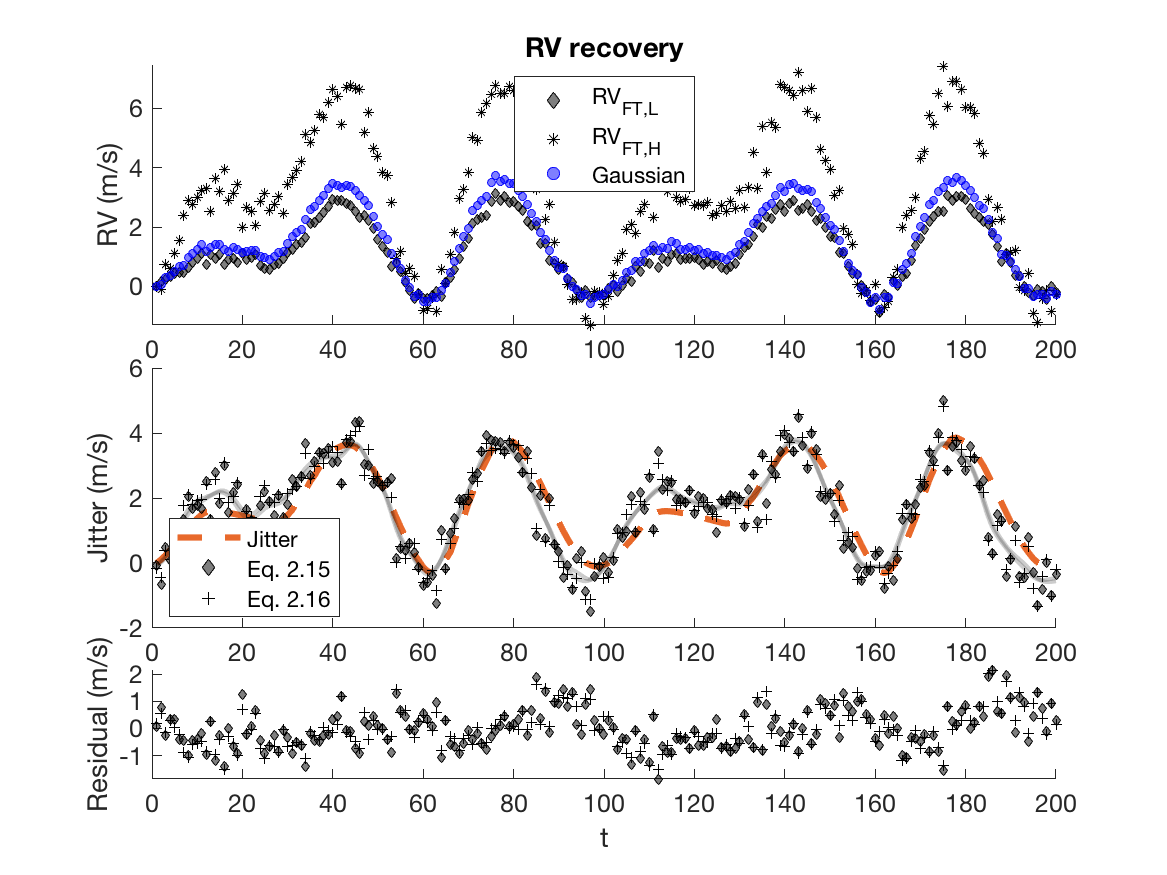
\includegraphics[width = 0.99 \linewidth]
{./Figures/Methods/5-PLANET_AND_JITTER.png}
\caption[Jitter model]
{Construct jitter model from simulation data.}
\label{fig:PLANET_AND_JITTER}
\end{figure} 
%-------------


\subsection{End-to-end Simulations}

Unless we are sure of a null-planetary system where $RV_\text{planet} = 0$ and
from Eq.~\ref{eq:RV_Gaussian} and Eq.~\ref{eq:RV_FT,L} we obtain
\begin{equation}
	k = RV_\text{jitter} / RV_\text{Gaussian},
\end{equation} 
normally $k$ cannot be directly calculated, so neither can $\alpha$ be.
However, we could substitute the jitter model (Eq.~\ref{eq:jitter_model}) into Eq.~\ref{eq:RV_Gaussian}, such that
\begin{equation}
	RV_\text{Gaussian} = RV_\text{planet} + \alpha \cdot \Delta RV
\label{eq:RV_fit}
\end{equation}
where $RV_\text{planet}$ is parametrised by Keplerian orbit(s) and both $RV_\text{Gaussian}$ and $\Delta RV$ 
are measurable. 

The tests are divided into two groups for comparison:
\begin{enumerate}
	\item Fit $RV_\text{Gaussian}$ by Keplerian orbit alone;
	\item Fit $RV_\text{Gaussian}$ by Keplerian orbit + jitter model (i.e. $\alpha \cdot \Delta RV$).
\end{enumerate}
The injected planet has the same parameter settings as in \S\ref{sec:check}, i.e. circular orbit with amplitude $A = 2$~m/s,
orbital frequency ratio $\nu = 0.7$ and initial phase $\omega = 1$~rad. We will compare which group recovers the 
planet parameters better. 

To better simulate the real observations, 40 data samples out of 200 from the two rotation periods are randomly selected.  
The fitting is achieved by running MCMC to maximise the log-likelihood function
given the model. For the simulation, each radial velocity data is equally weighted (as they have the same S/N). 
It is defined if the input parameter lies within $1\sigma$ errorbar of the output parameter, it counts as a 
successful detection. 

For demonstration, we show one of the outputs in corner plots (Fig.~\ref{fig:Corner}) and the corresponding 
radial velocity fitting (Fig.~\ref{fig:Planet_recovery}). The corner plot visually shows the how the walkers explore the parameter 
space and their distribution. The histogram gives an example explaining how a ``successful detection" is qualified. 
The radial velocity fitting plot demonstrates an example that implementing the jitter model effectively 
accounts for the spurious signals in the raw radial velocity data, reducing the rms from 1.14~m/s to 0.55~m/s. 

%-------------
\begin{figure}[tbp]
\centering
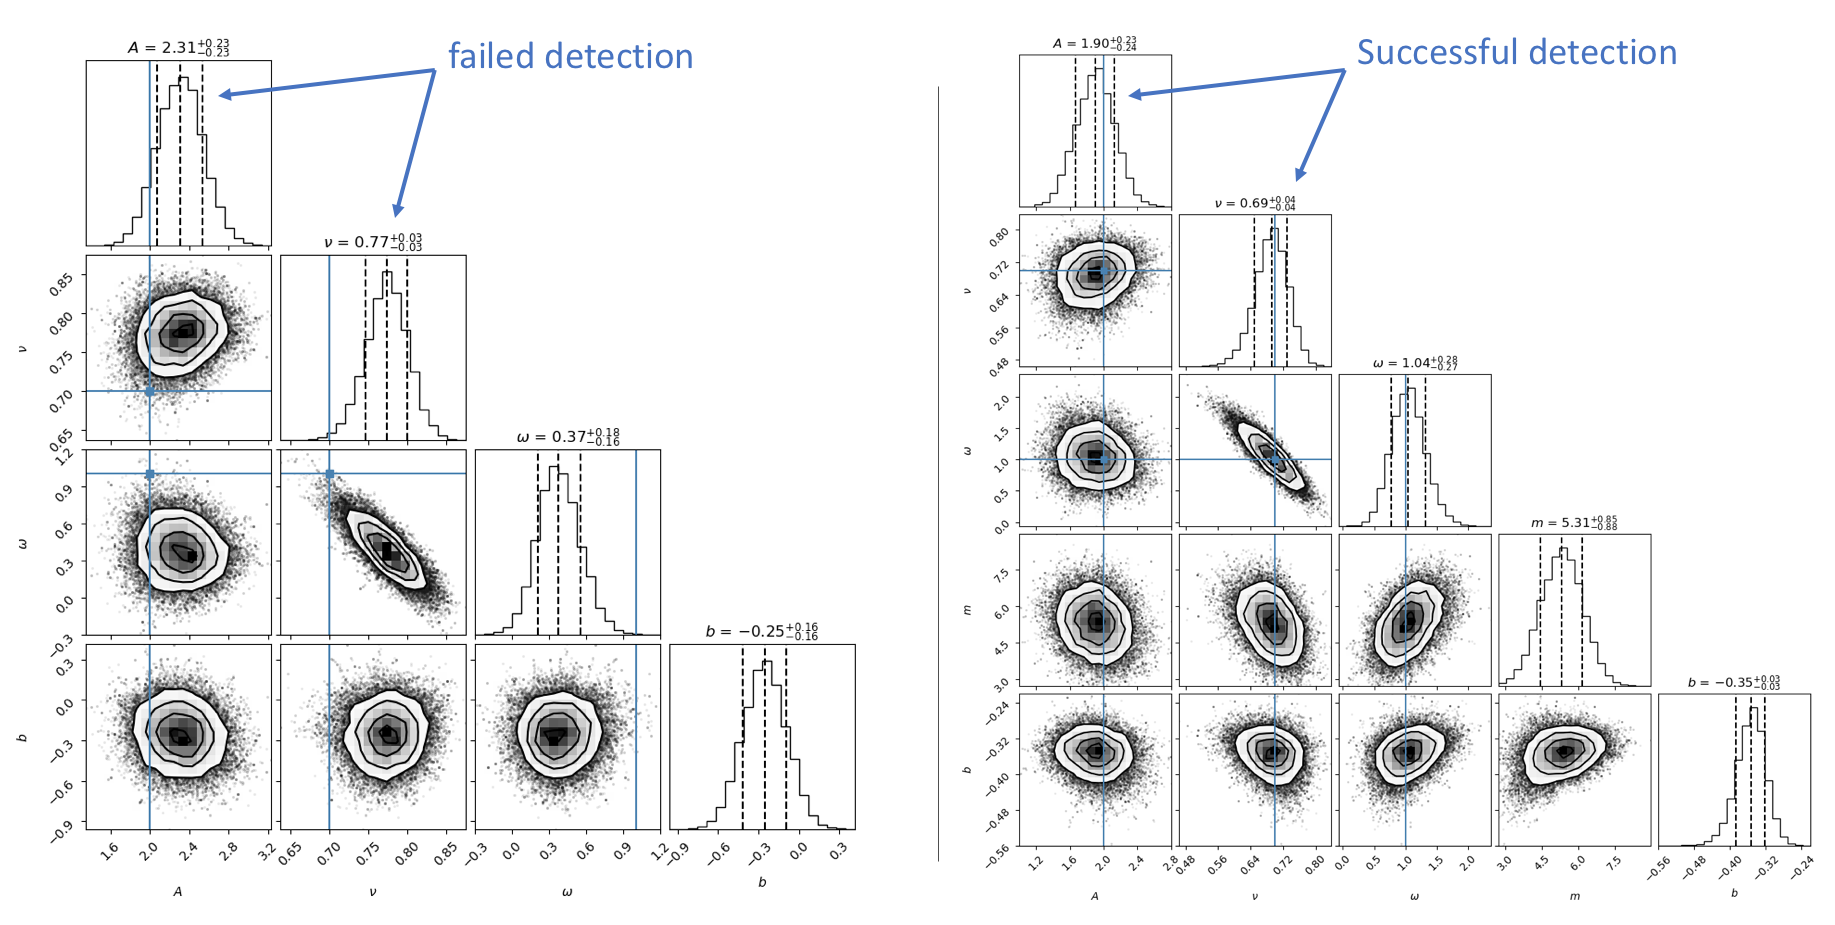
\includegraphics[width = 0.99 \linewidth]
{./Figures/Methods/Corner.png}
\caption[Corner plots of MCMC]
{Corner plots of MCMC. Theses are two examples of the output of MCMC: no jitter correction on the left and 
with jitter correction on the right. The input parameters are highlighted in the 
blue solid line. The three dashed lines of each histogram indicate the median and $1\sigma$ on both sides. On the 
left panel both blue lines of $A$ and $\nu$ are outside the $1\sigma$ region, therefore it counts as a ``failed detection";
on the right panel, it counts as a successful detection within $1\sigma$.}
\label{fig:Corner}
\end{figure} 
%-------------

%-------------
\begin{figure}[tbp]
\centering
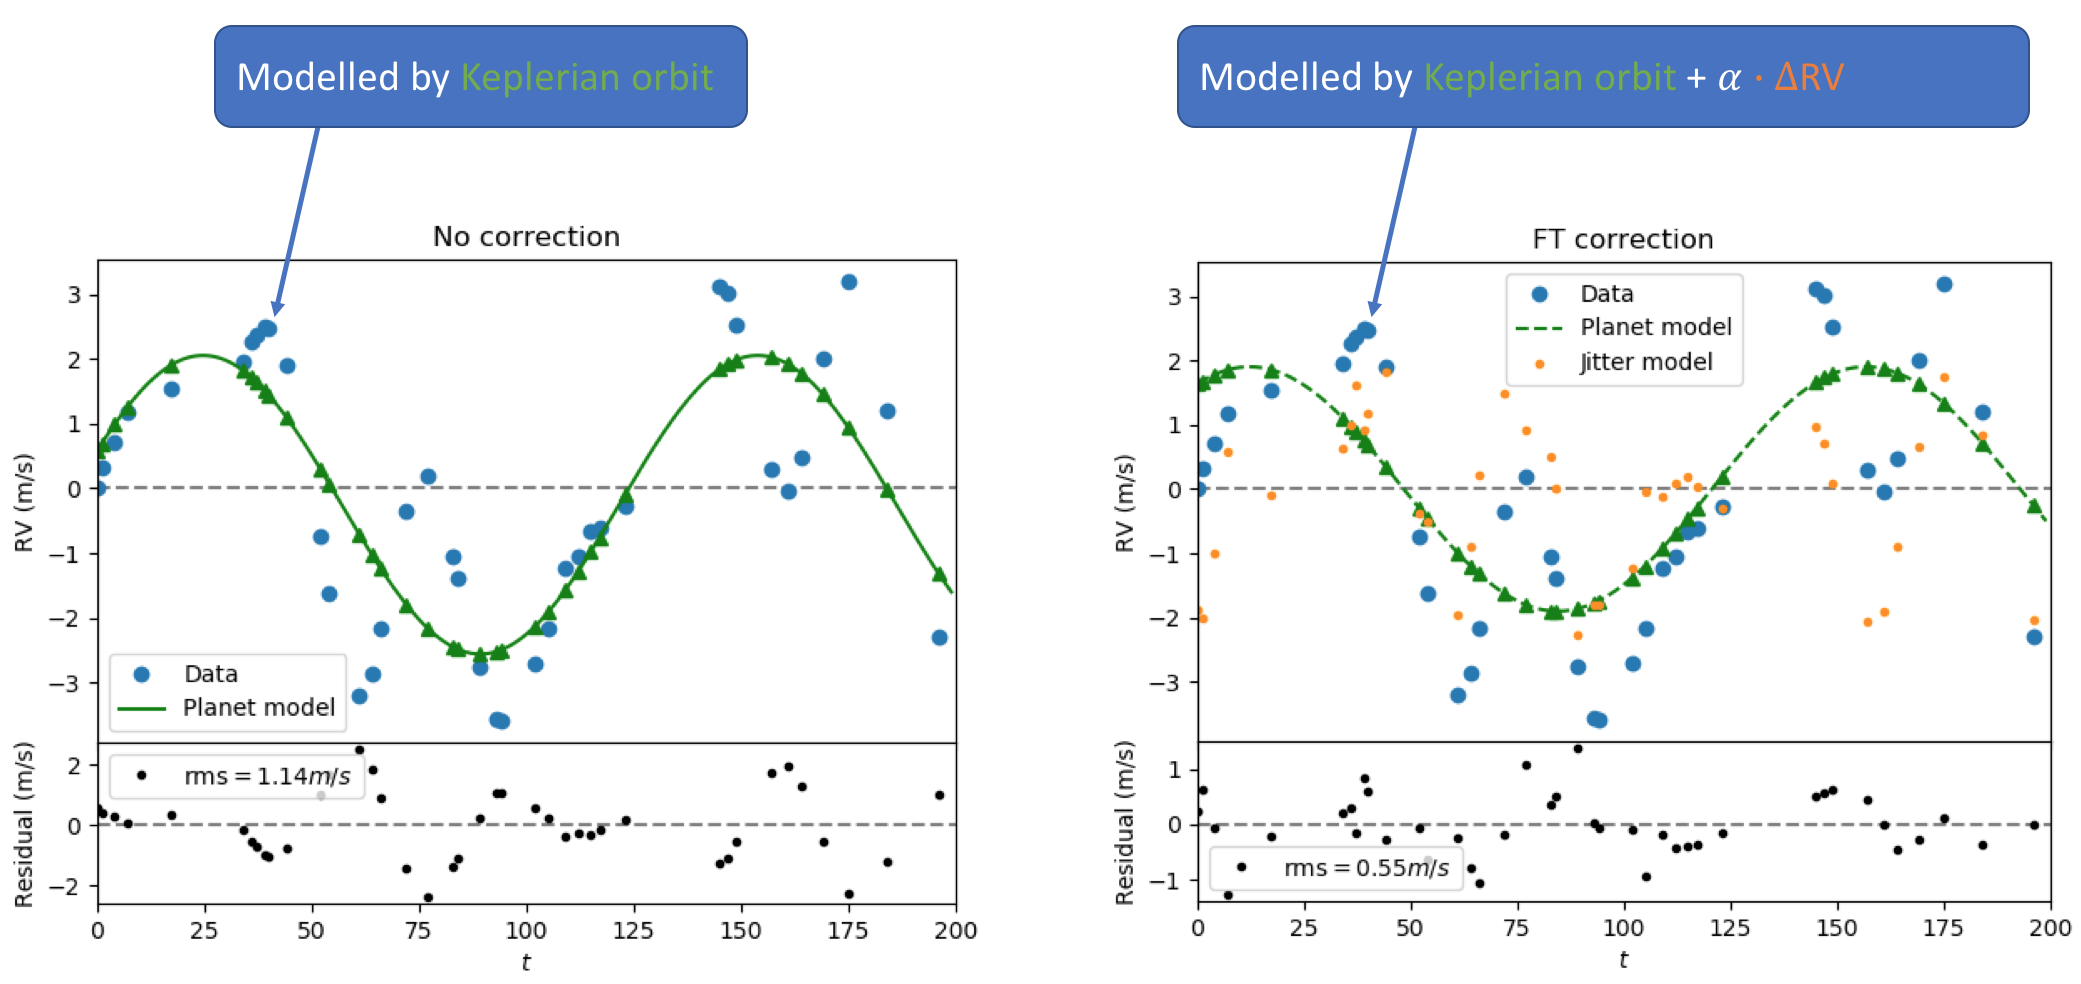
\includegraphics[width = 0.99 \linewidth]
{./Figures/Methods/Fitting.png}
\caption[Planet recovery]
{Radial velocity fitting. Theses are two fittings that comes out from the MCMC corner plots in Fig.~\ref{fig:Corner}. 
On the left panel without jitter correction, we can see that the input jitter increases the scatter of the raw radial 
velocities, resulting in an overestimated amplitude $A$; while on the right panel with jitter correction, the additional 
input jitter is accounted for by the jitter model.}
\label{fig:Planet_recovery}
\end{figure} 
%-------------

In the end, we run 100 trails for the end-to-end simulation. The random differences among these 100 trails come from:
\begin{itemize}
	\item photon noise given the S/N;
	\item randomly selected 40 samplings in the 200 line profiles.
\end{itemize}
It turns out that in $46\%$ of the 100 trails are successful detections for both $A$ and $\nu$ when we 
apply the jitter correction model, while this percentage is only $11\%$ without jitter correction. 
In more detail, Fig.~\ref{fig:FT_Statistics} shows that with jitter correction (in red), both of the amplitude and 
orbital frequency ratio tend to be underestimated, which is shown opposite for the results without correction (in blue). 
Moreover, the jitter corrected parameters are better constrained (i.e. with narrower distributions) and 
performs much better in $\nu$ than without correction. While it is tempting to say the correct answer is more likely in between
the results from these two fittings, we would need more tests to conclude. 

%-------------
\begin{figure}[tbp]	
    \begin{subfigure}[b]{0.49\textwidth}
        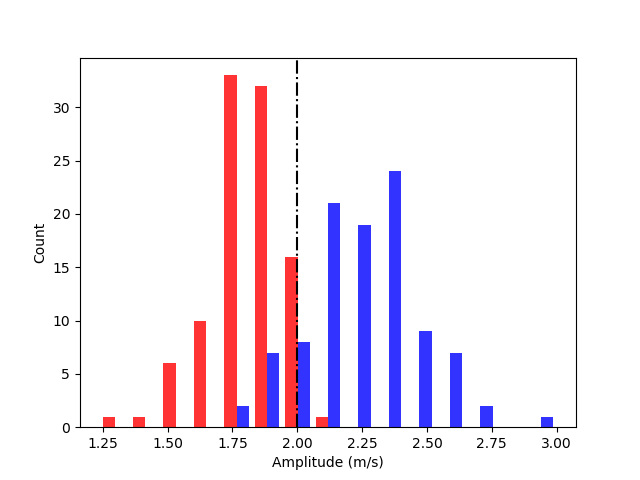
\includegraphics[width=\textwidth]{./Figures/Methods/Histogram_1.png}
        \caption{}
    \end{subfigure}
	~
    \begin{subfigure}[b]{0.49\textwidth}
        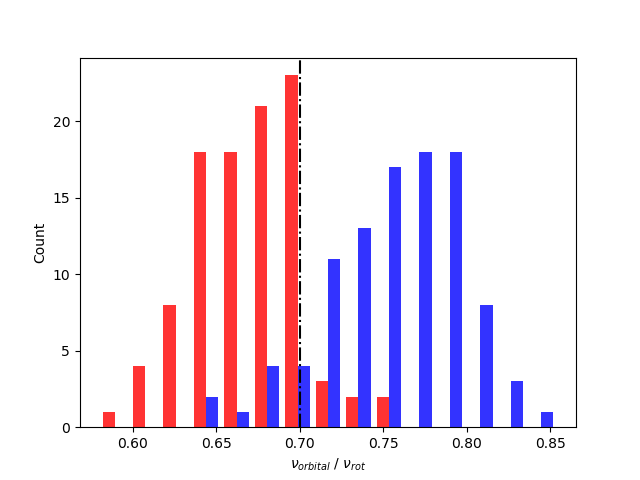
\includegraphics[width=\textwidth]{./Figures/Methods/Histogram_2.png}
        \caption{}
    \end{subfigure}	
    
    \caption[Distribution of recovered parameters]
    {Distribution of recovered parameters. The red are results of jitter correction by Fourier transform; 
    The blue are results of no jitter correction.}
\label{fig:FT_Statistics}
\end{figure}    
%-------------


%----------------------------------------------------------------------------------------
\section{Fourier transform with real observations}
\label{\thesection}
\label{sec:observation}

\subsection{HD189733: Rossiter–McLaughlin effect as jitter}

HD189733 is a well studied binary star system. The main star HD189733~A is known to host a gas giant
exoplanet HD189733~b, first detected by transits (reference...) and later by Doppler spectroscopy (references...). 
It was also the first exoplanet transit observed in X-ray (references...). 

We choose this target for the following reasons:
\begin{itemize}
	\item The exoplanet is well confirmed;
	\item The host star is bright enough: $m_v=7.66$
	\item The gas giant causes a prominent apparent radial velocity while it transits ($\sim 40$~m/s)
	due to Rossiter–McLaughlin effect.
\end{itemize}

%-------------
\begin{figure}[tbp]
\centering
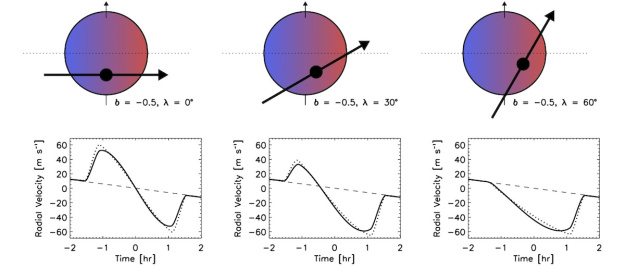
\includegraphics[width = 0.80 \linewidth]
{./Figures/Methods/rmeffect.jpg}
\caption[Demo: Rossiter–McLaughlin effect]
{Demo: Rossiter–McLaughlin effect (reference...). It is a apparent radial velocity
	change of the parent star due to an eclipsing binary (whether star or planet) that breaks the observed flux symmetry in the 
	stellar photosphere, resulting in imbalanced redshift and blueshift. It shows in this plot three different star-planet 
	alignments that causes three corresponding different shapes of radial velocity curve, and hence the radial velocity curve
	sheds information on the geometry of the alignment.}
\label{fig:rm-effect}
\end{figure} 
%-------------

We treat as if it were an ``active" star with one big dark starspot, as the Rossiter–McLaughlin effect 
causes the line profile deformed in a similar manner that a starspot would do (Fig.~\ref{fig:rm-effect}). 
We would see if our jitter model can account for the radial velocity variation from Rossiter–McLaughlin effect. 

The procedure is rather standardized. Both $RV_\text{Gaussian}$ and $RV_\text{FT}$ are calculated from the 
HARPS cross-correlation functions of the spectra. $\Delta RV = RV_\text{Gaussian} - RV_\text{FT}$ are then 
smoothed by a Gaussian filter (Fig.\ref{fig:hot_to_delta_rv}). The prototype of the Rossiter–McLaughlin
radial velocity curve is already identifiable in $\Delta RV$ of the lower panel. 

%-------------
\begin{figure}[tbp]
\centering
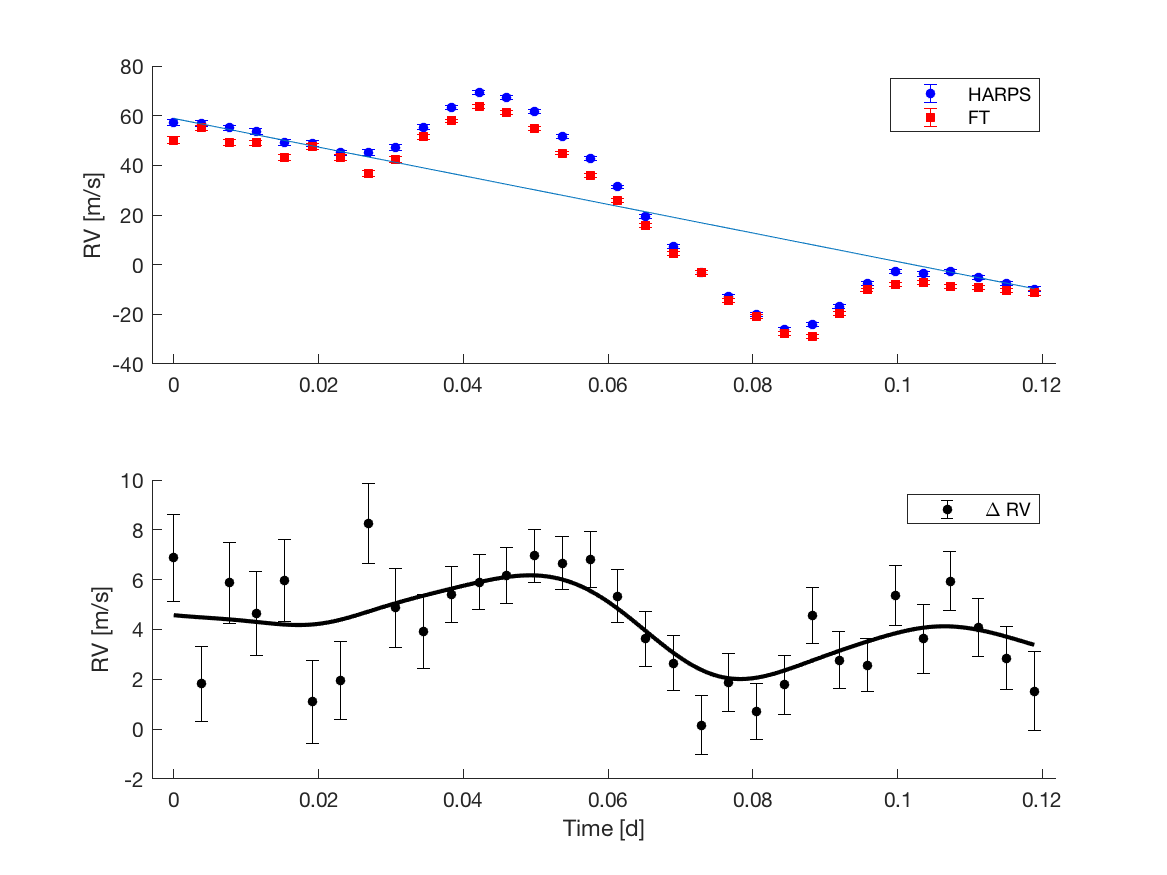
\includegraphics[width = 0.80 \linewidth]
{./Figures/Methods/8-Proto_jitter2.png}
\caption[From $RV_\text{Gaussian}$ and $RV_\text{FT}$ to $Delta RV$]
{From $RV_\text{Gaussian}$ and $RV_\text{FT}$ to $\Delta RV$. The scattered $\Delta RV$ are smoothed by applying 
a moving average with a Gaussian filter and  further weighted based on the size of errorbar.} 
\label{fig:hot_to_delta_rv}
\end{figure} 
%-------------

To extract the Rossiter–McLaughlin radial velocity curve, a linear trend is fitted to account for the 
other binary star. After the linear trend is removed, it is treated as jitter and modelled 
by $\alpha \cdot \Delta RV$ (Fig.~\ref{fig:rm_as_jitter}). 
Note that the errorbars of the jitter model also becomes a factor of $\alpha$ ($\alpha\gg 1$) larger; 
however, the model itself shows a descent approximation 
of the Rossiter–McLaughlin radial velocity curve. The peak of the ``jitter" is reduced from $\sim 40$~m/s to $\sim 10$~m/s. 

\paragraph{Remarks}
The effective length of the smoothing kernel should be carefully chosen. In this case, it's chosen most effective within 
roughly one neighbouring data point on both size. While mitigating the effect of noise (especially for relatively lower
S/N data outside the transits), to which the Fourier transform is sensitive, it also smears the drastic velocity 
change when the planet ingresses and egresses the stellar disk. To solve this awkward situation, an adaptive 
(i.e. S/N dependent) effective length of the smoothing kernel may be used. 

%-------------
\begin{figure}[tbp]
\centering
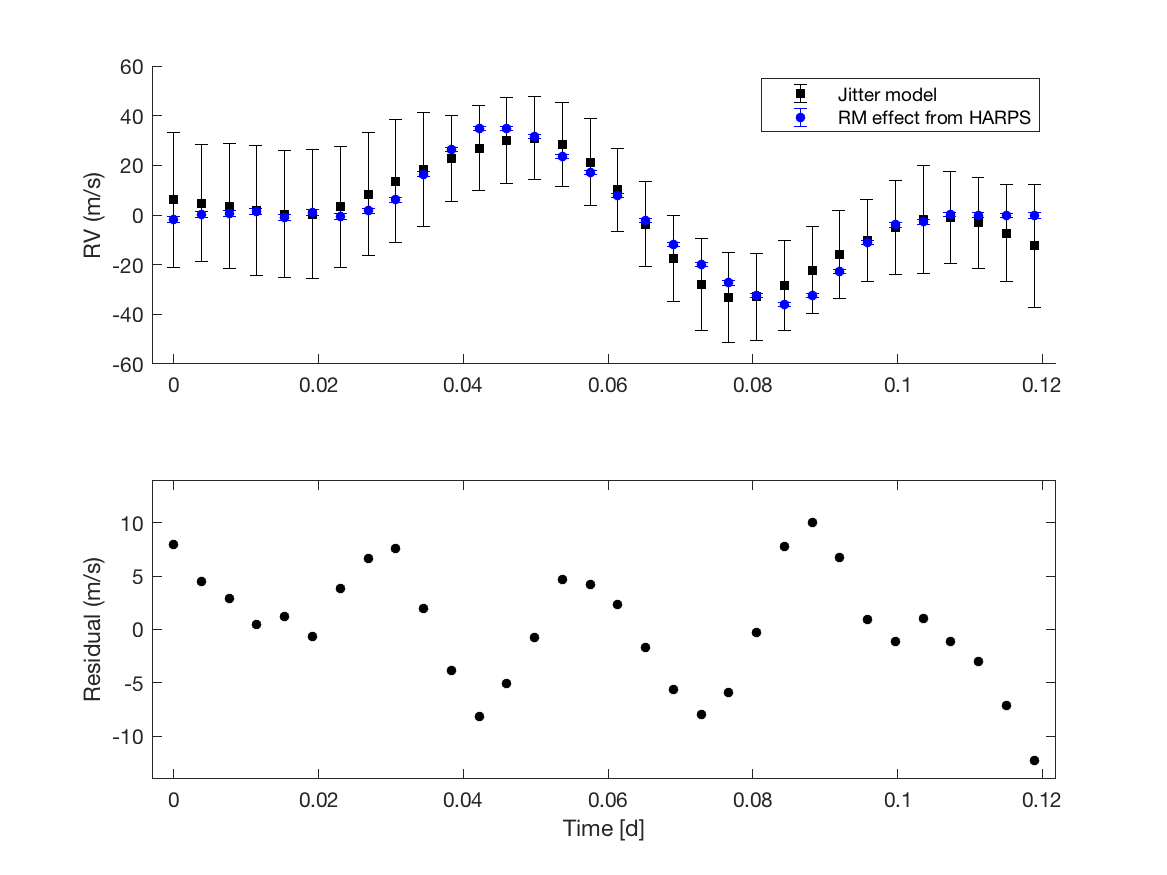
\includegraphics[width = 0.80 \linewidth]
{./Figures/Methods/9-RM_fit2.png}
\caption[Rossiter–McLaughlin effect as jitter]
{Rossiter–McLaughlin effect as jitter fitted with the jitter model.} 
\label{fig:rm_as_jitter}
\end{figure} 
%-------------

\subsection{Examples 2}

\subsection{Example 3}


%References like this: \cite{Selmeczi_07}


\FloatBarrier
A float barrier will stop figures from going beyond this point. They are handy to make sure they don't go into the next section.

%----------------------------------------------------------------------------------------
%\clearpage
\section{References}
\label{\thesection}
\vspace{-1.5cm}
\setstretch{1.0}
\bibliographystyle{unsrt}
\bibliography{Bibliography}
\setstretch{1.3}
